\documentclass[11pt,a4paper]{article}

\usepackage[T1]{fontenc}
\usepackage[utf8]{inputenc}
\usepackage{lmodern}
\usepackage[margin=2.5cm]{geometry}
\usepackage{microtype}
\usepackage{amsmath,amssymb}
\usepackage{booktabs,tabularx,multirow}
\usepackage{graphicx}
\usepackage{caption}
\usepackage{tikz}
\usetikzlibrary{arrows.meta,positioning}
\usepackage[hidelinks]{hyperref}
\usepackage{xcolor}

\graphicspath{{../recalc/figures/}}
\captionsetup{font=small,labelfont=bf}
\renewcommand{\arraystretch}{1.12}
\newcolumntype{Y}{>{\raggedright\arraybackslash}X}
\renewcommand{\tabularxcolumn}[1]{>{\raggedright\arraybackslash}p{#1}}

\newcommand{\nKO}{371}
\newcommand{\nSeasons}{13}
\newcommand{\nHome}{179}\newcommand{\nDraw}{72}\newcommand{\nAway}{120}
\newcommand{\drawEssay}{24.0\%}
\newcommand{\drawDC}{26.2\%}
\newcommand{\drawActual}{19.4\%}


\title{\textbf{Passing networks and Poisson goals}\\[4pt]
\large How far can probability and network theory go in analysing a football team?}
\author{Shaimay Shah\\[2pt]
\small Revised edition (2026) of an IB Mathematics Extended Essay (May 2018 session)}
\date{}

\begin{document}
\maketitle

\begin{abstract}
\noindent
This paper returns to the question I asked in my 2018 Extended Essay: \emph{how can the knowledge of probability and network theory help quantitatively and qualitatively analyse a football team?} I analyse the 2011 and 2015 UEFA Champions League finals, both won 3--1 by FC Barcelona. Passing data are modelled as weighted directed networks. I show that the 2018 centrality calculations treated the number of passes as a \emph{distance}, or ignored it entirely, and I redo them with the standard convention that more passes means a shorter distance. The corrected results reverse the original essay's main conclusion. Barcelona in 2011 were not an evenly spread passing team: 91\% of their betweenness belonged to three players, and removing Xavi alone would cut the team's passing efficiency by 14\%. I then extend the analysis with a player-removal (``red card'') test, community detection, comparisons with random networks and a bootstrap of the rankings. For the probability model, I fix an inconsistency in the league averages and remove the final itself from the data used to predict it. I then test the model on \nKO{} Champions League knockout matches. It forecasts no better than simply using the season's home, draw and away rates; adding home advantage, and fitting a Dixon--Coles model, both improve on it. Finally, event data from StatsBomb give players' real positions and the quality of every chance (expected goals, xG), which links the two halves of the essay. In 2011 Barcelona created 1.93 xG to Manchester United's 0.30, a performance that would win about 80\% of the time. In 2015, when Barcelona played through their right-hand side, the players at the centre of the passing network were also the players who built the chances.
\end{abstract}

\section*{Preface to this edition}
I wrote the original essay when I was eighteen. Re-reading it, I found the idea sound but several calculations wrong. Mathematica's centrality functions use edge weights as lengths, so the heaviest passing links became the longest paths. The ``league average'' used for goals scored differed from the one used for goals conceded, which is impossible. The statistics used to predict each final also contained the final's own result. This edition keeps the research question and the two-part structure. It corrects every calculation, adds the tests the original essay called for but never carried out, and brings in better data. All numbers in the tables are produced by the code published alongside this paper, and Section~\ref{sec:reproducibility} explains how to rerun it. The recalculation and extension were carried out with the help of Claude, an AI assistant made by Anthropic.

\tableofcontents
\newpage

%=====================================================================
\section{Introduction}
%=====================================================================

Football is the world's most watched sport, and for a long time it was one of the least quantified. Its flow is continuous. Goals are rare. Much of what makes a team good, such as how it keeps the ball, moves it and creates chances, never shows up in simple counts like goals and assists. Companies such as Opta and StatsBomb now record every pass and shot, so a match can be treated as data.

Two branches of mathematics fit this data naturally. \textbf{Network theory} treats players as nodes and passes as weighted, directed edges. Measures developed for social networks, the web and transport systems can then describe a team's structure: who the ball flows through, who is easy to reach, and which groups of players combine. \textbf{Probability} treats goals as rare, random events. A Poisson model then turns estimates of attacking and defensive strength into probabilities for every possible score.

I apply both to two matches that make a useful pair: the Champions League finals of 2011 (Barcelona 3--1 Manchester United, at Wembley) and 2015 (Juventus 1--3 Barcelona, in Berlin). Barcelona won both 3--1, but they played very differently. The research question is unchanged from 2018:

\begin{quote}
\emph{How can the knowledge of probability and network theory help quantitatively and qualitatively analyse a football team?}
\end{quote}

\noindent Compared with the original essay, this edition:
\begin{enumerate}
  \item corrects the centrality calculations and shows exactly how the original values arose (Section~\ref{sec:2018});
  \item adds team-level measures, a player-removal test and passing units (Sections~\ref{sec:team}--\ref{sec:units});
  \item checks whether the network patterns could arise by chance, and how stable the player rankings are (Section~\ref{sec:significance});
  \item corrects the Poisson model and tests it on \nKO{} matches instead of two (Sections~\ref{sec:poisson}--\ref{sec:test});
  \item uses StatsBomb event data to place players at their real positions, split the matches by half, measure chance quality with expected goals and link the network to the chances created (Sections~\ref{sec:positions}--\ref{sec:link}).
\end{enumerate}

%=====================================================================
\section{Data}\label{sec:data}
%=====================================================================

\paragraph{Passing tables (Opta).} The 2018 essay used Opta's passing data for the starting eleven of each team in each final: the number of completed passes from every player to every other player over the whole match. Substitutes are left out, so every network has the same eleven nodes. The four $11\times 11$ tables are reproduced in Appendix~\ref{app:matrices}.

\paragraph{Event data (StatsBomb).} StatsBomb's free Open Data release \cite{statsbomb} includes both finals. It records every on-ball event: over 1{,}200 passes in the 2011 final and almost 1{,}000 in 2015, each with a location, recipient and outcome, as well as every shot with its expected-goals value. I use it to check the Opta tables, to find the players' real positions and to measure the quality of the chances.

\paragraph{Results (openfootball).} To test the probability model on more than two matches, I use every Champions League result from 2011/12 to 2023/24, taken from the public-domain openfootball dataset \cite{openfootball}. These are \nSeasons{} seasons with 96 group-stage matches and 23--29 knockout matches each. The 2010/11 season is not in this dataset.

\paragraph{Do the sources agree?} Table~\ref{tab:sbcheck} compares the Opta tables used in 2018 with the same passes counted from StatsBomb's events. The totals differ by at most nine passes. Across all 110 possible passing links, the correlation is at least 0.98 for three teams and 0.92 for Juventus. The original data were therefore transcribed accurately, and none of the corrections below come from bad data.

\begin{table}[t]
\centering\small
\caption{Opta passing tables against StatsBomb event data: completed passes between starters, and the correlation between the two sources over all 110 possible passing links.}
\label{tab:sbcheck}
\begin{tabular}{lrrrr}
\toprule
Team & StatsBomb formation & Opta & StatsBomb & Correlation \\
\midrule
Barça 2011 & 4-1-2-2-1 & 707 & 716 & 1.00 \\
Man Utd 2011 & 4-2-2-2 & 262 & 256 & 0.98 \\
Barça 2015 & 4-1-2-2-1 & 512 & 510 & 0.99 \\
Juventus 2015 & 4-1-2-1-2 & 276 & 278 & 0.92 \\
\bottomrule
\end{tabular}
\end{table}


%=====================================================================
\section{Network theory}\label{sec:networks}
%=====================================================================

\subsection{Passing networks}

A team's passing in a match is represented by a \textbf{weighted directed graph} with the eleven starters as nodes. Its \textbf{adjacency matrix} $A$ has entries
\[
A_{xy} = \text{number of completed passes from player } x \text{ to player } y, \qquad A_{xx} = 0 .
\]
The graph is directed because $A_{xy}$ and $A_{yx}$ usually differ: goalkeepers pass far more to centre-backs than centre-backs pass back. The weight of the edge $x\to y$ measures the \emph{strength} of the link. The total number of passes a player makes, $L^{\text{out}}_x = \sum_y A_{xy}$, is their \textbf{out-strength}. Figure~\ref{fig:networks} draws the four networks with players at their positions in each team's formation.

\begin{figure}[p]
\centering
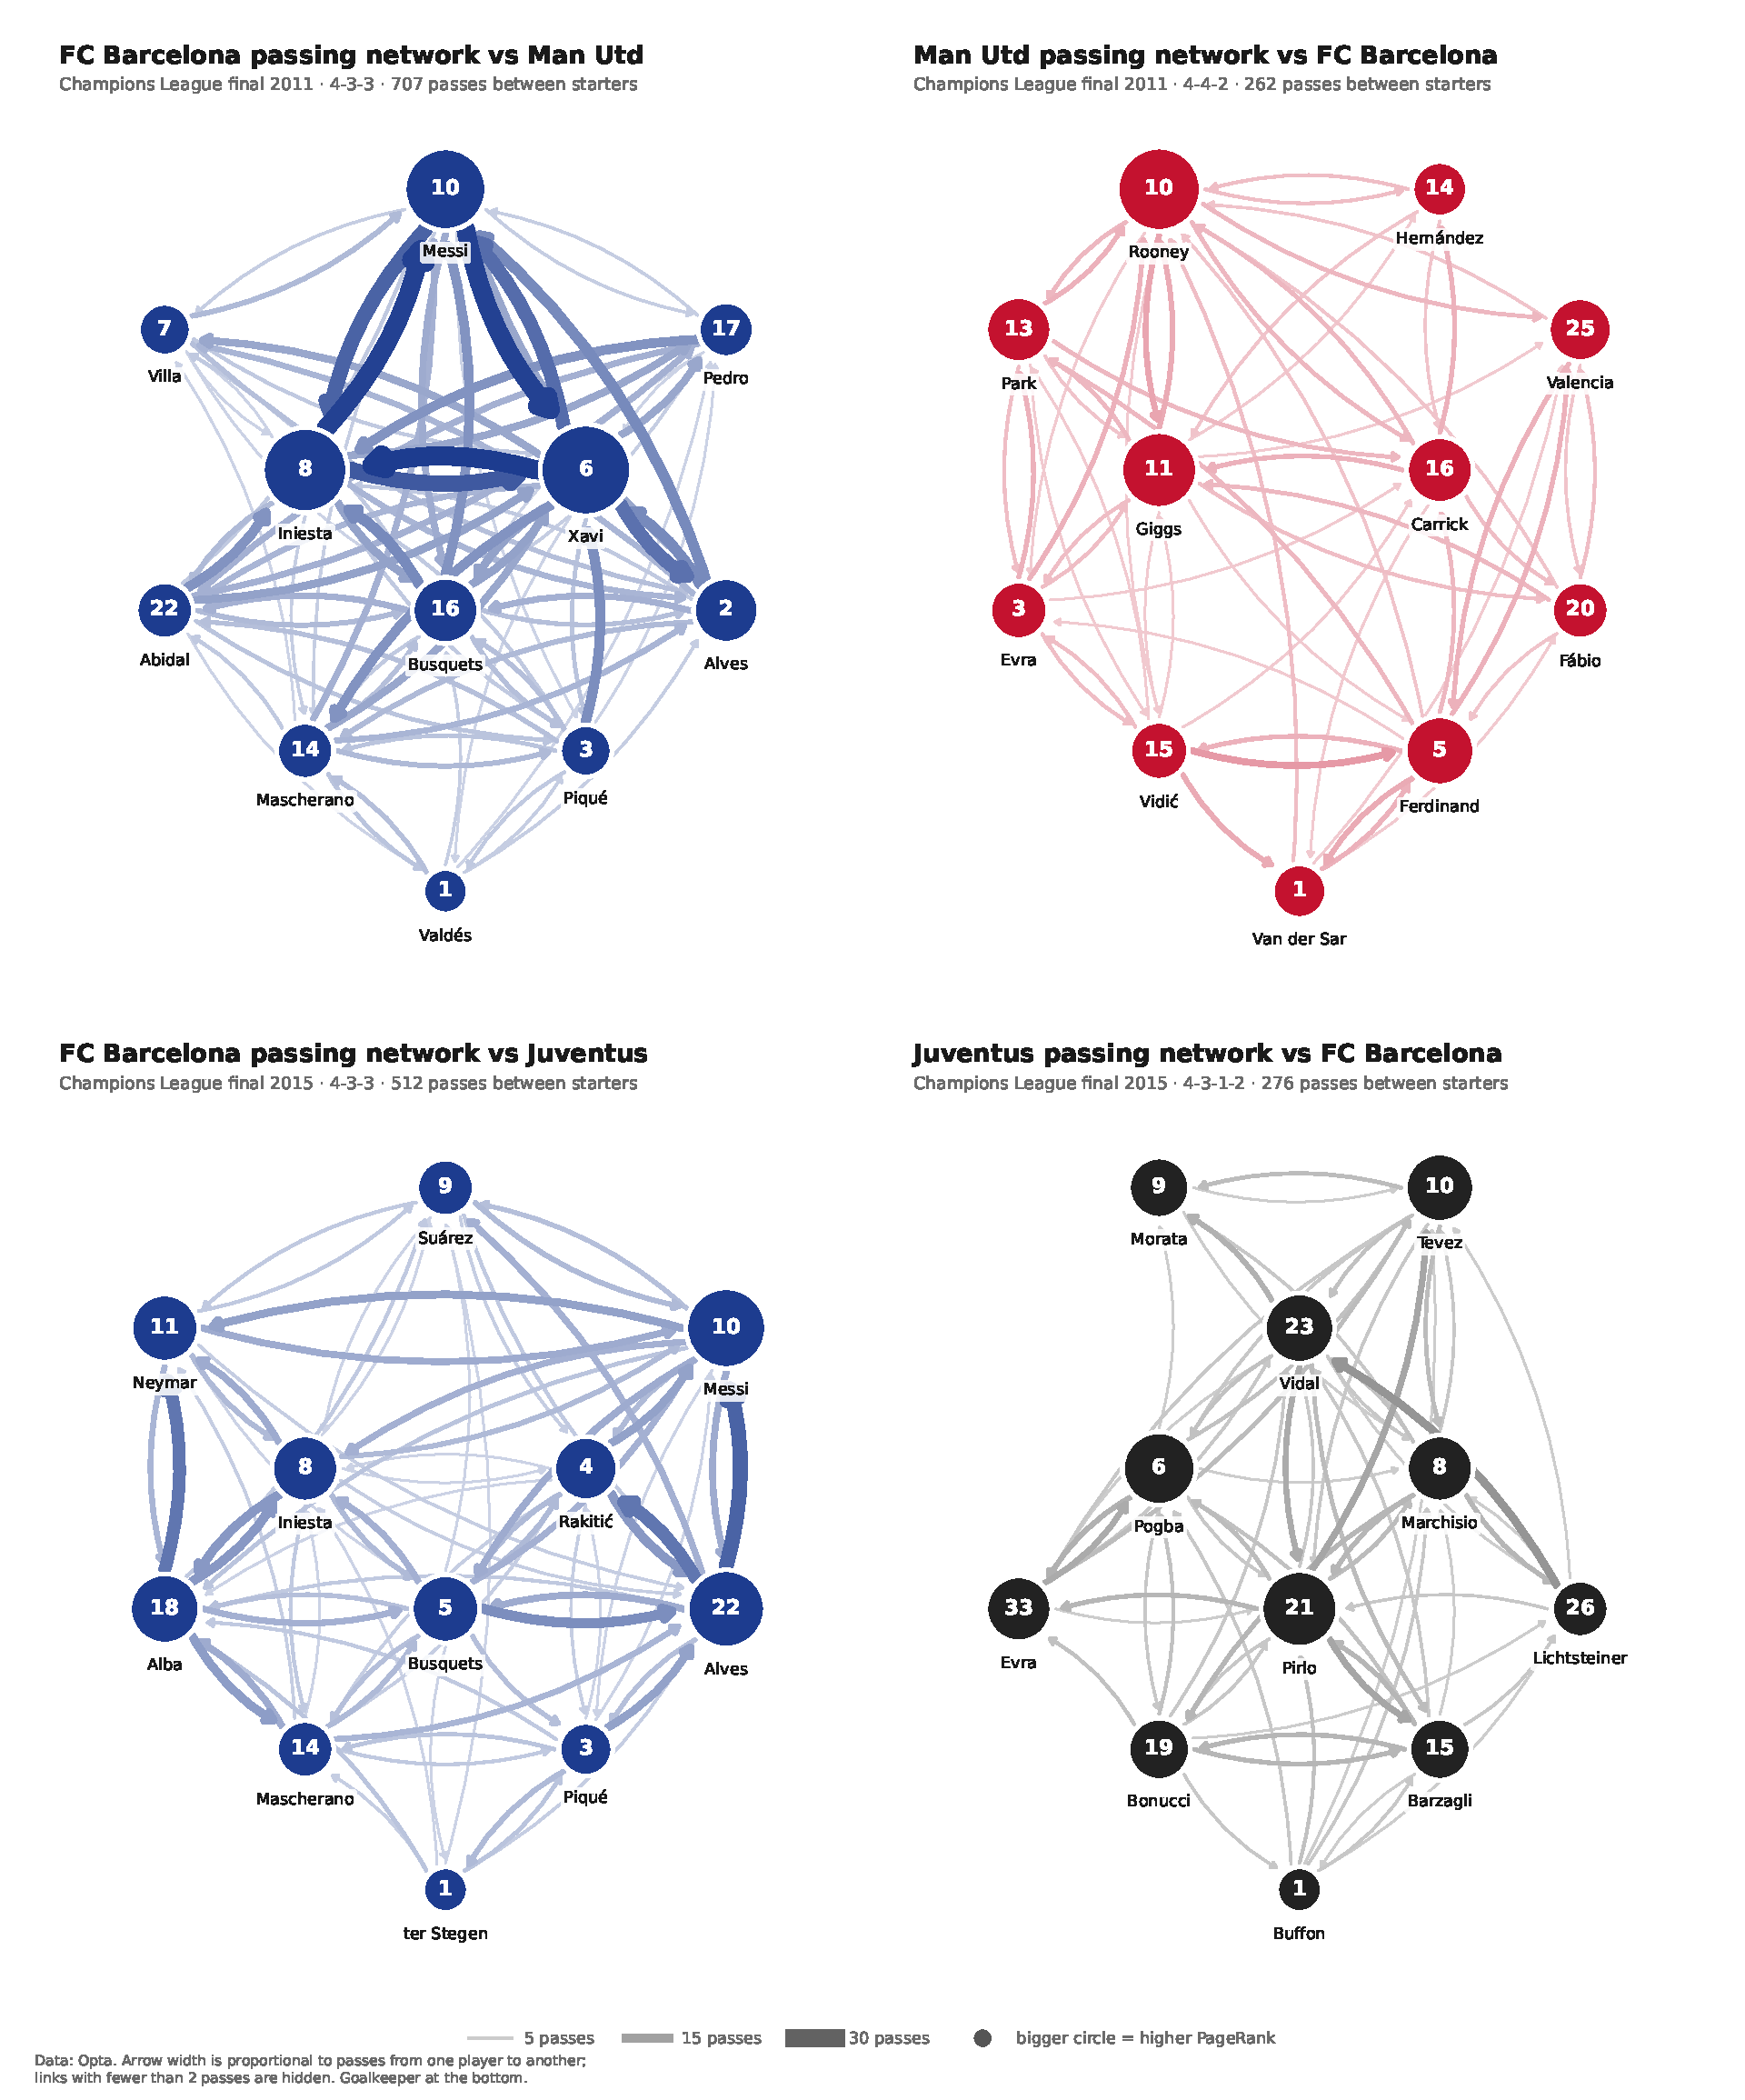
\includegraphics[width=\textwidth]{all_networks.pdf}
\caption{The four passing networks (Opta), redrawn from the 2018 essay. Arrow width is proportional to the number of passes; circle size shows weighted PageRank. The original figures scaled arrow thickness with the \emph{square} of the number of passes, which turned Barcelona's midfield into solid black shapes. Here the scale is linear and the same for all four teams.}
\label{fig:networks}
\end{figure}

\subsection{Strength and distance}\label{sec:distance}

Several measures rely on \textbf{shortest paths} (geodesics): the cheapest route for the ball from one player to another. For that we need the \emph{length} of each edge. A link used 30 times should be \emph{shorter} than a link used twice, because the ball travels along it easily. The standard choice, and the one used by L\'opez Pe\~na and Touchette \cite{pena} whose method the 2018 essay followed, is
\[
d_{xy} = \frac{1}{A_{xy}} \qquad (A_{xy} > 0),
\]
and the length of a path is the sum of the lengths of its edges. The geodesic distance $D_{xy}$ is the length of the shortest path from $x$ to $y$.

Figure~\ref{fig:toy} shows why this matters. Player A passes to B 30 times, and passes to B via C only twice on each leg. If the number of passes is used as the length, the direct route costs $30$ and the detour costs $2+2=4$. The ``shortest'' path then avoids the busiest link in the team, and C is credited with holding the team together. With $d = 1/A$, the direct route costs $1/30 \approx 0.03$ against $1/2+1/2 = 1$ for the detour, which is the sensible answer.

\begin{figure}[t]
\centering
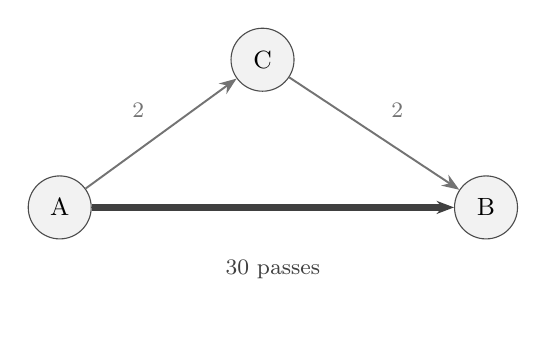
\begin{tikzpicture}[>={Stealth[length=2.2mm]}, node distance=2.4cm,
  every node/.style={circle, draw=black!70, fill=black!5, minimum size=8mm, font=\small}]
  \node (A) {A};
  \node (B) [right=4.6cm of A] {B};
  \node (C) [above right=1.3cm and 2cm of A] {C};
  \draw[->, line width=2.4pt, black!75] (A) -- node[below, draw=none, fill=none, font=\footnotesize] {30 passes} (B);
  \draw[->, line width=0.7pt, black!55] (A) -- node[above left, draw=none, fill=none, font=\footnotesize] {2} (C);
  \draw[->, line width=0.7pt, black!55] (C) -- node[above right, draw=none, fill=none, font=\footnotesize] {2} (B);
\end{tikzpicture}
\caption{Treating passes as distances turns the network upside down. With length $=$ passes, the shortest route from A to B goes through C ($2+2 < 30$). With length $= 1/\text{passes}$ it is the direct link ($1/30 < 1/2 + 1/2$).}
\label{fig:toy}
\end{figure}

\subsection{Player measures}

\paragraph{Betweenness centrality} measures how much of the ball's flow between other players depends on player $x$ \cite{freeman, brandes}:
\[
C_B(x) = \frac{1}{(N-1)(N-2)} \sum_{y \ne x \ne z} \frac{n^x_{yz}}{g_{yz}},
\]
where $g_{yz}$ is the number of geodesics from $y$ to $z$ and $n^x_{yz}$ the number of those passing through $x$. With $N = 11$ the normalising factor is $1/90$, so $0 \le C_B(x) \le 1$. A high value means that isolating the player (by marking, or a red card) would disrupt the team's passing.

\paragraph{Closeness centrality} is the reciprocal of a player's average geodesic distance to the others:
\[
C_C(x) = \frac{N-1}{\sum_{y \ne x} D_{xy}} .
\]
Because distances are measured in units of $1/\text{passes}$, closeness is measured in passes. It is larger for teams that pass more, so it should only be compared between players in the same team.

\paragraph{PageRank} \cite{brin} treats a player as important if important players pass to them often. The scores solve
\[
x_i = \frac{1-p}{N} + p \sum_{j} \frac{A_{ji}}{L^{\text{out}}_j}\, x_j , \qquad \sum_i x_i = 1,
\]
with $p = 0.85$. $x_i$ can be read as the long-run share of time the ball spends with player $i$ if it follows passes at random, with probability $1-p$ of restarting from a random player. (The 2018 essay wrote $A_{xy}$ in place of $A_{ji}$, which runs the passes the wrong way.)

\paragraph{Weighted clustering} measures how often a player's passing partners also pass to each other, forming triangles. For directed weighted graphs I use Fagiolo's generalisation \cite{fagiolo} of the Onnela et al.\ formula \cite{onnela} quoted in 2018:
\[
c^w_i = \frac{\big[(\hat W^{1/3} + (\hat W^{T})^{1/3})^3\big]_{ii}}{2\big[k_i(k_i-1) - 2k^{\leftrightarrow}_i\big]}, \qquad \hat W = \frac{A}{\max A},
\]
where the powers $1/3$ are taken entry by entry, $k_i$ is the number of distinct players $i$ passes to or receives from (counting each direction), and $k^{\leftrightarrow}_i$ the number of two-way links. Dividing by $\max A$ means only triangles of heavy links score highly. The 2018 formula divided by the number of passes where it needed the number of links.

\subsection{Team measures}\label{sec:teamdefs}

The 2018 methodology promised ``global network invariants'' for the team as a whole but never calculated any. I use the following.
\begin{itemize}
\item \textbf{Density}: the share of the $N(N-1) = 110$ possible links used at least once.
\item \textbf{Reciprocity}: $\sum_{x,y}\min(A_{xy},A_{yx}) / \sum_{x,y} A_{xy}$, the share of passes that were returned along the same link.
\item \textbf{Passing entropy}: $H = -\sum p_{xy}\ln p_{xy} / \ln 110$ with $p_{xy} = A_{xy}/\sum A$. It equals 1 if passes are spread evenly over all links and is lower if a few links dominate.
\item \textbf{Betweenness centralisation} \cite{freeman}: $\sum_x \big(\max_y C_B(y) - C_B(x)\big)/(N-1)$. It equals 1 for a ``star'' in which every route runs through one player, and 0 when all players have equal betweenness.
\item \textbf{Global efficiency} \cite{latora}: $E = \frac{1}{N(N-1)}\sum_{x\ne y} 1/D_{xy}$, the average ease of moving the ball between two players. Dividing $E$ by the team's average weight per link gives a \emph{relative efficiency} that does not simply reward teams for passing more.
\item \textbf{Modularity} \cite{newman}: how well the team splits into ``passing units'' that pass mainly among themselves (Section~\ref{sec:units}).
\end{itemize}

\subsection{A note on the 2018 calculations}\label{sec:2018}

All four 2018 measures were computed with Mathematica's built-in functions. I can reproduce every published value from the passing tables, and doing so shows exactly what went wrong (Table~\ref{tab:reproduction}):
\begin{itemize}
\item \textbf{Closeness} matches to three decimal places when the number of passes is used as the \emph{distance}. The busiest players therefore looked the most distant. Xavi and Busquets came out least central, and the essay concluded that Barcelona ``isn't extremely well connected''.
\item \textbf{Betweenness} and \textbf{PageRank} match exactly when the weights are \emph{ignored}. One pass counted the same as 33, and the values were not normalised by $1/90$ as the essay's formula stated.
\item \textbf{Clustering} is close to, but does not exactly match, an unweighted calculation.
\end{itemize}
In other words, the pass counts entered the pictures but hardly entered the mathematics. Everything that follows uses the corrected definitions.

\begin{table}[t]
\centering\small
\caption{Reproducing the 2018 results for Barça 2011. Closeness is reproduced exactly when the number of passes is used as a \emph{distance}; betweenness is reproduced exactly when the weights are ignored. The corrected values use $d_{xy} = 1/A_{xy}$.}
\label{tab:reproduction}
\begin{tabular}{lrrrrrr}
\toprule
 & \multicolumn{3}{c}{Closeness} & \multicolumn{3}{c}{Betweenness} \\
\cmidrule(lr){2-4}\cmidrule(lr){5-7}
Player & 2018 & passes as distance & corrected & 2018 & unweighted & corrected \\
\midrule
Valdés & 0.400 & 0.400 & 3.33 & 0.536 & 0.536 & 0.000 \\
Piqué & 0.500 & 0.500 & 7.31 & 1.590 & 1.594 & 0.000 \\
Mascherano & 0.244 & 0.244 & 6.50 & 2.590 & 2.592 & 0.183 \\
Alves & 0.435 & 0.435 & 6.73 & 1.230 & 1.225 & 0.000 \\
Abidal & 0.333 & 0.333 & 6.64 & 1.390 & 1.392 & 0.000 \\
Xavi & 0.227 & 0.227 & 9.59 & 3.130 & 3.127 & 0.567 \\
Busquets & 0.189 & 0.189 & 6.95 & 1.860 & 1.861 & 0.000 \\
Iniesta & 0.233 & 0.233 & 8.06 & 1.860 & 1.861 & 0.111 \\
Pedro & 0.313 & 0.312 & 5.82 & 0.583 & 0.583 & 0.000 \\
Messi & 0.345 & 0.345 & 7.84 & 1.570 & 1.569 & 0.089 \\
Villa & 0.286 & 0.286 & 3.95 & 0.661 & 0.661 & 0.000 \\
\bottomrule
\end{tabular}
\end{table}


%=====================================================================
\section{Results: the passing networks}\label{sec:results}
%=====================================================================

\subsection{Players}

Table~\ref{tab:centralities} lists the corrected measures for every player. Three results stand out.

\textbf{Barcelona 2011 ran through Xavi.} Xavi has the highest betweenness (0.567), closeness, PageRank and clustering in his team. Only four Barcelona players have any betweenness at all. The top three by PageRank are Xavi, Iniesta and Messi. This is the trio the 2018 essay, from the pictures alone, suggested Manchester United should have tried to isolate.

\textbf{Manchester United's play ran from centre-back to striker.} Ferdinand has the highest betweenness and closeness, and Rooney the highest PageRank. This is the long-ball route from defence to attack visible in Figure~\ref{fig:networks}. The 2018 essay named Giggs, Carrick, Valencia and Rooney as United's ``backbone''. The corrected numbers keep Rooney and Giggs but replace Carrick and Valencia with Ferdinand.

\textbf{In 2015 Barcelona's centre moved to the right flank.} Alves and Messi top both betweenness and PageRank. The 2018 essay argued for a shift ``from control in the midfield to playing through the wings'' using \emph{Juventus's} PageRank scores. That comparison is invalid, because PageRank sums to one within each team. Barcelona's own numbers now support the claim directly. For Juventus, Pirlo has the highest betweenness, closeness and PageRank, followed by Marchisio and Vidal. The 2018 conclusion that the defenders Bonucci and Lichtsteiner were the key players, and that Juventus were therefore ``on the back foot'', does not survive the correction.

\begin{table}[p]
\centering
\caption{Corrected player measures from the Opta passing tables, sorted by PageRank. $C_B$ = normalised betweenness, $C_C$ = closeness (in units of passes), PR = weighted PageRank ($p = 0.85$), $c^w$ = weighted clustering.}
\label{tab:centralities}

\begin{minipage}[t]{0.48\textwidth}\centering\footnotesize
\textbf{Barça 2011}\\[2pt]
\begin{tabular}{lrrrr}
\toprule
Player & $C_B$ & $C_C$ & PR & $c^w$ \\
\midrule
Xavi & 0.567 & 9.59 & 0.178 & 0.227 \\
Iniesta & 0.111 & 8.06 & 0.157 & 0.207 \\
Messi & 0.089 & 7.84 & 0.149 & 0.214 \\
Busquets & 0.000 & 6.95 & 0.097 & 0.179 \\
Alves & 0.000 & 6.73 & 0.094 & 0.189 \\
Abidal & 0.000 & 6.64 & 0.067 & 0.171 \\
Mascherano & 0.183 & 6.50 & 0.066 & 0.137 \\
Pedro & 0.000 & 5.82 & 0.062 & 0.146 \\
Villa & 0.000 & 3.95 & 0.052 & 0.116 \\
Piqué & 0.000 & 7.31 & 0.051 & 0.120 \\
Valdés & 0.000 & 3.33 & 0.028 & 0.085 \\
\bottomrule
\end{tabular}
\end{minipage}\hfill
\begin{minipage}[t]{0.48\textwidth}\centering\footnotesize
\textbf{Man Utd 2011}\\[2pt]
\begin{tabular}{lrrrr}
\toprule
Player & $C_B$ & $C_C$ & PR & $c^w$ \\
\midrule
Rooney & 0.222 & 3.22 & 0.154 & 0.233 \\
Giggs & 0.106 & 2.81 & 0.130 & 0.206 \\
Ferdinand & 0.243 & 3.56 & 0.108 & 0.242 \\
Carrick & 0.106 & 2.70 & 0.097 & 0.186 \\
Park & 0.006 & 2.65 & 0.095 & 0.222 \\
Valencia & 0.067 & 2.64 & 0.088 & 0.185 \\
Vidić & 0.074 & 3.09 & 0.072 & 0.230 \\
Evra & 0.026 & 3.10 & 0.070 & 0.247 \\
Fábio & 0.000 & 2.46 & 0.067 & 0.257 \\
Hernández & 0.000 & 1.96 & 0.061 & 0.254 \\
Van der Sar & 0.011 & 2.65 & 0.058 & 0.206 \\
\bottomrule
\end{tabular}
\end{minipage}

\vspace{10pt}

\begin{minipage}[t]{0.48\textwidth}\centering\footnotesize
\textbf{Barça 2015}\\[2pt]
\begin{tabular}{lrrrr}
\toprule
Player & $C_B$ & $C_C$ & PR & $c^w$ \\
\midrule
Messi & 0.267 & 5.49 & 0.143 & 0.193 \\
Alves & 0.267 & 6.50 & 0.135 & 0.187 \\
Alba & 0.111 & 5.56 & 0.110 & 0.174 \\
Busquets & 0.144 & 6.43 & 0.103 & 0.191 \\
Neymar & 0.011 & 4.28 & 0.102 & 0.170 \\
Iniesta & 0.067 & 4.68 & 0.098 & 0.143 \\
Rakitić & 0.000 & 4.91 & 0.089 & 0.156 \\
Suárez & 0.000 & 3.24 & 0.068 & 0.115 \\
Mascherano & 0.000 & 5.25 & 0.067 & 0.122 \\
Piqué & 0.144 & 5.72 & 0.056 & 0.118 \\
ter Stegen & 0.000 & 3.52 & 0.029 & 0.105 \\
\bottomrule
\end{tabular}
\end{minipage}\hfill
\begin{minipage}[t]{0.48\textwidth}\centering\footnotesize
\textbf{Juventus 2015}\\[2pt]
\begin{tabular}{lrrrr}
\toprule
Player & $C_B$ & $C_C$ & PR & $c^w$ \\
\midrule
Pirlo & 0.256 & 3.72 & 0.130 & 0.212 \\
Pogba & 0.028 & 2.40 & 0.120 & 0.172 \\
Vidal & 0.139 & 3.20 & 0.109 & 0.234 \\
Tevez & 0.109 & 2.83 & 0.106 & 0.202 \\
Marchisio & 0.163 & 3.52 & 0.098 & 0.189 \\
Evra & 0.011 & 2.34 & 0.095 & 0.203 \\
Bonucci & 0.083 & 2.76 & 0.084 & 0.166 \\
Barzagli & 0.094 & 3.12 & 0.082 & 0.195 \\
Morata & 0.000 & 1.39 & 0.080 & 0.148 \\
Lichtsteiner & 0.009 & 2.88 & 0.067 & 0.153 \\
Buffon & 0.000 & 2.40 & 0.029 & 0.164 \\
\bottomrule
\end{tabular}
\end{minipage}
\end{table}


\subsection{Teams}\label{sec:team}

Table~\ref{tab:global} summarises each team in single numbers. Barcelona 2011 stands out. Its betweenness centralisation is 0.53, against about 0.19 for the other three teams, and its involvement inequality is the highest. Its low modularity says it played as one connected block rather than in separate units. It also made more than 2.5 times as many passes as United.

This reverses the central claim of the 2018 essay, that Barcelona had ``a low and consistent betweenness score which implies that there is less reliance on individual skill''. Barcelona 2011 was the \emph{most} dependent of the four teams on a single player. That dependence was on a midfielder who touched the ball constantly, not on one who dribbled past people.

\begin{table}[t]
\centering\small
\caption{Team-level network measures (Opta passing tables).}
\label{tab:global}
\begin{tabular}{lrrrr}
\toprule
Measure & Barça 2011 & Man Utd 2011 & Barça 2015 & Juventus 2015 \\
\midrule
Completed passes between starters & 707 & 262 & 512 & 276 \\
Density & 0.85 & 0.75 & 0.82 & 0.78 \\
Reciprocity & 0.79 & 0.69 & 0.72 & 0.59 \\
Passing entropy (normalised) & 0.882 & 0.894 & 0.887 & 0.900 \\
Betweenness centralisation & 0.528 & 0.181 & 0.192 & 0.192 \\
Betweenness held by top three & 91\% & 66\% & 67\% & 62\% \\
Involvement inequality (Gini) & 0.311 & 0.175 & 0.211 & 0.162 \\
PageRank inequality (Gini) & 0.284 & 0.174 & 0.200 & 0.157 \\
Mean weighted clustering & 0.163 & 0.224 & 0.152 & 0.185 \\
Relative efficiency & 1.35 & 1.39 & 1.37 & 1.33 \\
Modularity of passing units & 0.056 & 0.156 & 0.152 & 0.093 \\
\bottomrule
\end{tabular}
\end{table}


\subsection{The red-card test}\label{sec:redcard}

Betweenness only counts shortest paths. A more direct question is: \emph{how much harder does it become for the other players to pass to each other if one player is removed?} For each player $x$, I compute the global efficiency among the other ten players with and without $x$ available as an intermediary:
\[
\Delta_x = 1 - \frac{E_{\text{without } x}(\text{others})}{E_{\text{with } x}(\text{others})} .
\]
Averaging over the same pairs in both cases means $\Delta_x \ge 0$, and it measures only $x$'s role as a link. The same calculation removes pairs and trios. Table~\ref{tab:redcard} and Figure~\ref{fig:redcard} show the results.

Removing Xavi costs Barcelona 2011 14\% of its efficiency. No other player in that team is above 3\%. The trio the 2018 essay suggested isolating (Xavi, Iniesta, Messi) causes a 23\% drop, the 9th largest of the 165 possible trios\unskip. That is a good choice, but Xavi, Busquets and Iniesta does more damage (31\%). For the other teams the dependence is spread more evenly. Barcelona 2015 relied most on the right-back Alves (7\%). Juventus relied equally on Pirlo and Vidal.

\begin{table}[t]
\centering\small
\caption{The red-card test: fall in passing efficiency between the remaining players when a player, pair or trio is removed.}
\label{tab:redcard}
\begin{tabularx}{\textwidth}{lXXX}
\toprule
Team & Most needed players & Most damaging pair & Most damaging trio \\
\midrule
Barça 2011 & Xavi (14\%), Iniesta (3\%) & Xavi + Iniesta (23\%) & Xavi + Busquets + Iniesta (31\%) \\
Man Utd 2011 & Ferdinand (6\%), Rooney (3\%) & Ferdinand + Rooney (16\%) & Ferdinand + Giggs + Rooney (28\%) \\
Barça 2015 & Alves (7\%), Messi (4\%) & Alba + Alves (15\%) & Alba + Alves + Messi (25\%) \\
Juventus 2015 & Pirlo (4\%), Vidal (4\%) & Pirlo + Vidal (10\%) & Bonucci + Pirlo + Vidal (18\%) \\
\bottomrule
\end{tabularx}
\end{table}


\begin{figure}[t]
\centering
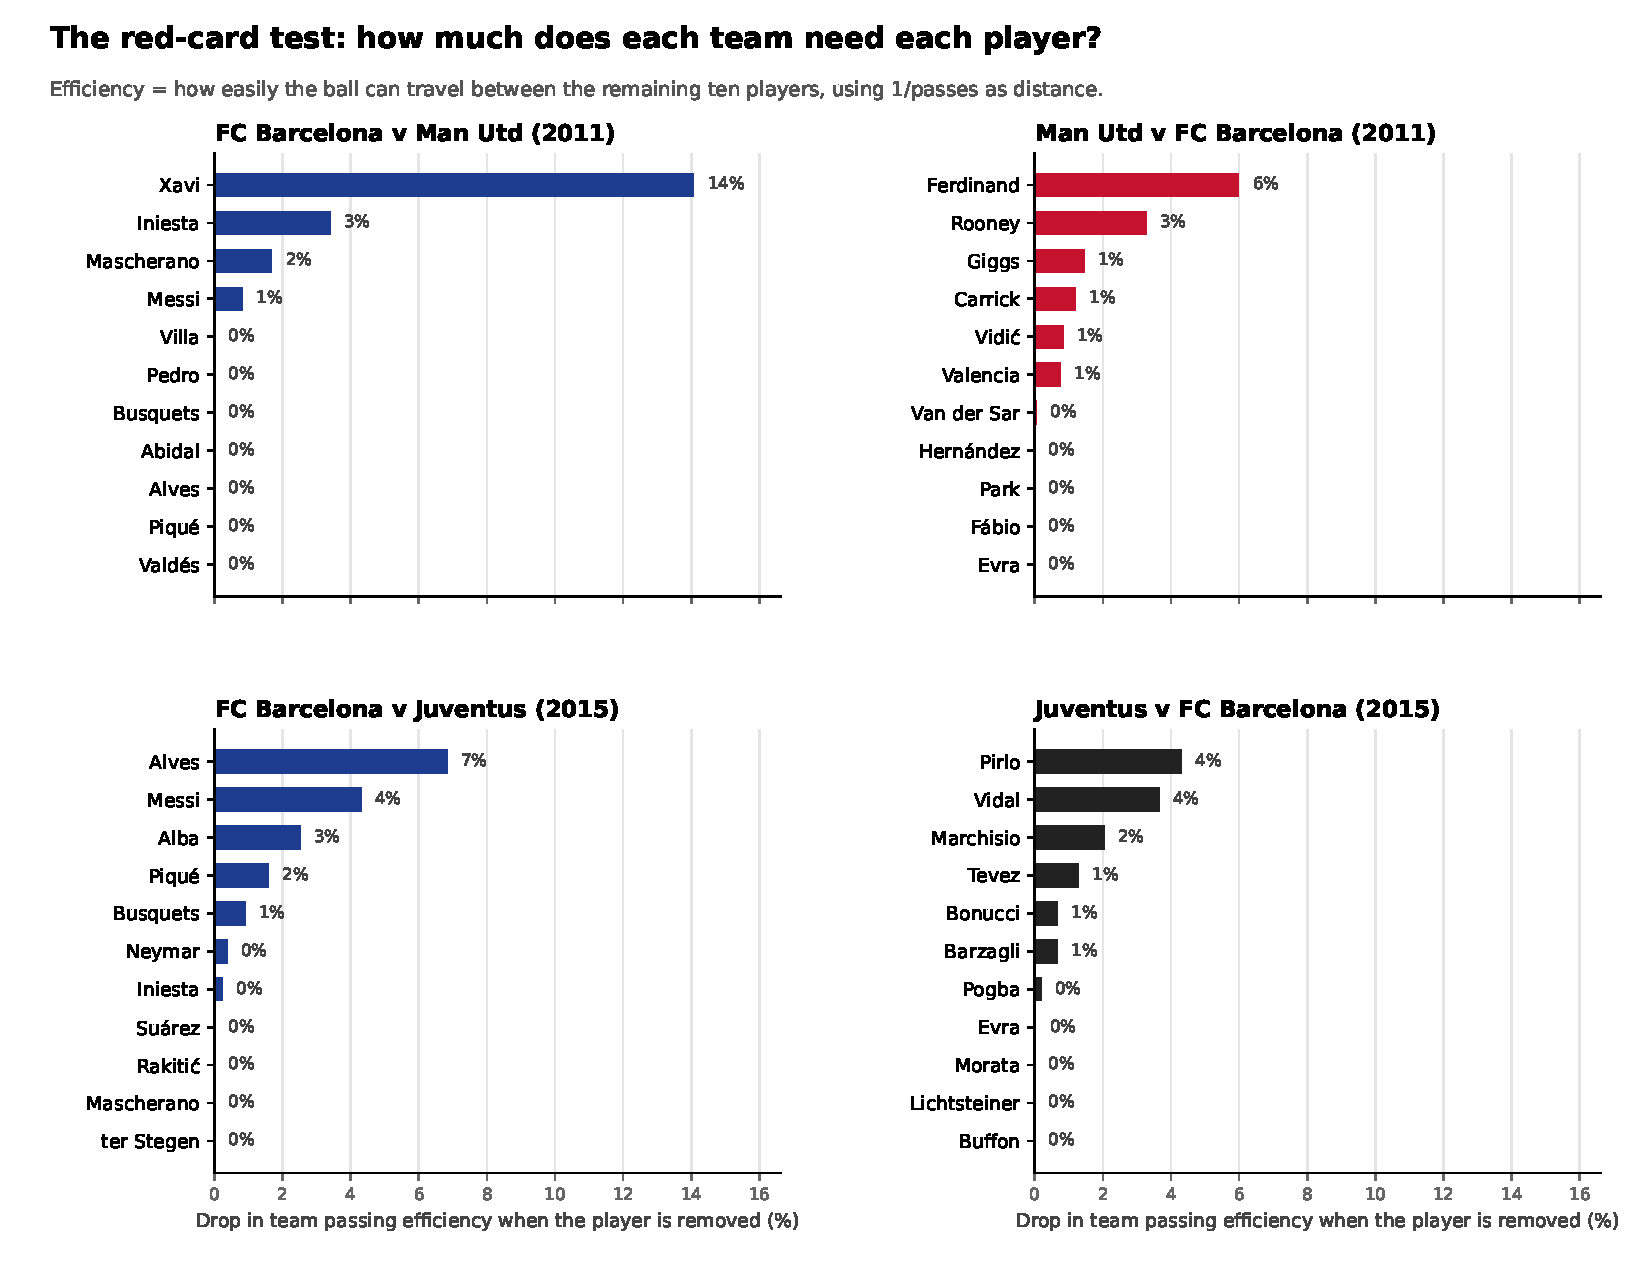
\includegraphics[width=\textwidth]{red_card.pdf}
\caption{The red-card test for every player: the fall in passing efficiency between the remaining ten players when the player is removed.}
\label{fig:redcard}
\end{figure}

\subsection{Passing units}\label{sec:units}

Community detection looks for groups of players who pass mainly among themselves. I combine passes in both directions and maximise the modularity
\[
Q = \frac{1}{2m}\sum_{x,y}\Big(w_{xy} - \frac{s_x s_y}{2m}\Big)\,\delta(c_x, c_y),
\]
where $w_{xy} = A_{xy} + A_{yx}$, $s_x$ is player $x$'s total passes, $2m = \sum_{x,y} w_{xy}$ and $\delta(c_x,c_y) = 1$ if $x$ and $y$ are in the same group. The maximisation uses the Louvain algorithm \cite{louvain}, keeping the best of 20 runs. Table~\ref{tab:units} lists the groups.

Barcelona 2011 has almost no structure ($Q = 0.056$). Six players (Alves, Busquets, Xavi, Iniesta, Messi and Villa) form a single unit. The centre-backs and goalkeeper form a second group, and Abidal and Pedro a small left-sided pair. Barcelona 2015 splits clearly into a right side (Alves, Busquets, Rakiti\'c, Messi, Su\'arez) and a left side (Alba, Iniesta, Mascherano, Neymar). This is the most direct evidence for the change in style between the two finals. Manchester United divide into a left-sided and attacking group (Evra, Park, Giggs, Carrick, Rooney, Hern\'andez) and a right-sided and defensive group (Van der Sar, the centre-backs, F\'abio and Valencia). This fits both their long passes forward and Valencia's deep position (Section~\ref{sec:positions}).

\begin{table}[t]
\centering\small
\caption{Passing units found by Louvain community detection (passes in both directions combined).}
\label{tab:units}
\begin{tabularx}{\textwidth}{lrX}
\toprule
Team & $Q$ & Units \\
\midrule
Barça 2011 & 0.056 & Alves, Busquets, Iniesta, Messi, Villa, Xavi; Mascherano, Piqué, Valdés; Abidal, Pedro \\
Man Utd 2011 & 0.156 & Carrick, Evra, Giggs, Hernández, Park, Rooney; Ferdinand, Fábio, Valencia, Van der Sar, Vidić \\
Barça 2015 & 0.152 & Alves, Busquets, Messi, Rakitić, Suárez; Alba, Iniesta, Mascherano, Neymar; Piqué, ter Stegen \\
Juventus 2015 & 0.093 & Barzagli, Bonucci, Buffon, Pirlo; Lichtsteiner, Marchisio, Morata, Vidal; Evra, Pogba, Tevez \\
\bottomrule
\end{tabularx}
\end{table}


\subsection{Could these patterns be chance?}\label{sec:significance}

A busy player will look central in almost any network, simply because they have more passes to spread around. To separate \emph{who passed to whom} from \emph{how much each player passed}, I compare each team with 1{,}000 random networks. In each one, every player makes and receives exactly as many passes as in the real match, but the receivers are shuffled at random, with no player passing to himself. If a real value lies far outside the random ones, it reflects genuine structure.

Table~\ref{tab:null} gives the results as $z$-scores. Three findings are clear. First, \textbf{modularity} and \textbf{passing entropy} are far from random for every team: real teams concentrate their passes on particular links and form genuine units. Second, real teams are more \textbf{efficient} than random ones with the same pass totals. Third, \textbf{betweenness centralisation} is \emph{not} unusual. Barcelona's reliance on Xavi is fully explained by the number of passes he made and received, not by any special position in the network. The random comparison ignores the pitch, so a goalkeeper is as likely to pass to a striker as to a centre-back. It is a demanding baseline, and the clearest results should be read with that in mind.

\begin{table}[t]
\centering\small
\caption{Real networks compared with 1000 random networks per team that keep every player's number of passes made and received. Entries are $z$-scores (standard deviations from the random mean); $^{*}$ marks $p < 0.05$ (two-sided).}
\label{tab:null}
\begin{tabular}{lrrrr}
\toprule
Measure & Barça 2011 & Man Utd 2011 & Barça 2015 & Juventus 2015 \\
\midrule
Reciprocity & $-0.5$ & $+0.8$ & $-1.3$ & $-1.9$ \\
Passing entropy & $-13.8$$^{*}$ & $-7.2$$^{*}$ & $-19.5$$^{*}$ & $-6.4$$^{*}$ \\
Betweenness centralisation & $-0.4$ & $-0.7$ & $-0.9$ & $-1.3$ \\
Top-three betweenness share & $-2.7$ & $-1.8$ & $-2.8$$^{*}$ & $-2.2$$^{*}$ \\
Mean weighted clustering & $-0.4$ & $-1.0$ & $-4.0$$^{*}$ & $-2.6$$^{*}$ \\
Relative efficiency & $+4.5$$^{*}$ & $+5.9$$^{*}$ & $+11.3$$^{*}$ & $+4.3$$^{*}$ \\
Modularity & $+15.5$$^{*}$ & $+9.2$$^{*}$ & $+19.3$$^{*}$ & $+4.6$$^{*}$ \\
\bottomrule
\end{tabular}
\end{table}


\paragraph{How stable are the rankings?} The pass counts are themselves noisy. A slightly different game could have produced a few more or a few fewer passes on each link. I resample every entry of $A$ from a Poisson distribution with mean $A_{xy}$, 1{,}000 times, and record who comes out on top (Table~\ref{tab:bootstrap}). Xavi tops betweenness in 99\% of resamples and the red-card test in 100\%. In contrast, the order of Rooney and Ferdinand at United, and of Alves and Messi at Barcelona in 2015, changes often. These players are best described as ``joint most important'' rather than ranked.

\begin{table}[t]
\centering\small
\caption{How often each player comes out on top when every pass count is resampled 1000 times from a Poisson distribution centred on the observed count (players topping fewer than 5\% of resamples omitted).}
\label{tab:bootstrap}
\begin{tabularx}{\textwidth}{lXXX}
\toprule
Team & Top betweenness & Top PageRank & Top in red-card test \\
\midrule
Barça 2011 & Xavi 99\% & Xavi 87\%, Iniesta 11\% & Xavi 100\% \\
Man Utd 2011 & Rooney 50\%, Ferdinand 33\%, Giggs 12\% & Rooney 79\%, Giggs 17\% & Ferdinand 49\%, Rooney 37\%, Giggs 9\% \\
Barça 2015 & Alves 65\%, Messi 22\%, Busquets 6\%, Alba 6\% & Messi 68\%, Alves 29\% & Alves 76\%, Messi 17\%, Alba 5\% \\
Juventus 2015 & Pirlo 64\%, Vidal 13\%, Marchisio 12\% & Pirlo 51\%, Pogba 27\%, Vidal 9\%, Tevez 7\% & Pirlo 59\%, Vidal 25\%, Marchisio 7\% \\
\bottomrule
\end{tabularx}
\end{table}


\subsection{Real positions}\label{sec:positions}

The 2018 networks placed players at fixed positions in their formation, a limitation the essay noted itself. StatsBomb's event data let each player be placed at the average location of their passes and receptions (Figure~\ref{fig:sbnetworks}). Several things become visible that a formation diagram hides:
\begin{itemize}
\item Barcelona 2011 squeezed into a compact block in the opponent's half, with both full-backs level with the halfway line.
\item Manchester United's right winger Valencia played almost exactly level with right-back F\'abio, in effect as a second full-back. StatsBomb records United's shape as 4-2-2-2, not the 4-4-2 used in 2018.
\item Barcelona 2015 is visibly split into the left and right units found in Section~\ref{sec:units}, with Busquets between them.
\end{itemize}
Because the StatsBomb passing counts match Opta so closely (Table~\ref{tab:sbcheck}), every player ranking in this section is unchanged when recalculated from StatsBomb data.

\begin{figure}[p]
\centering
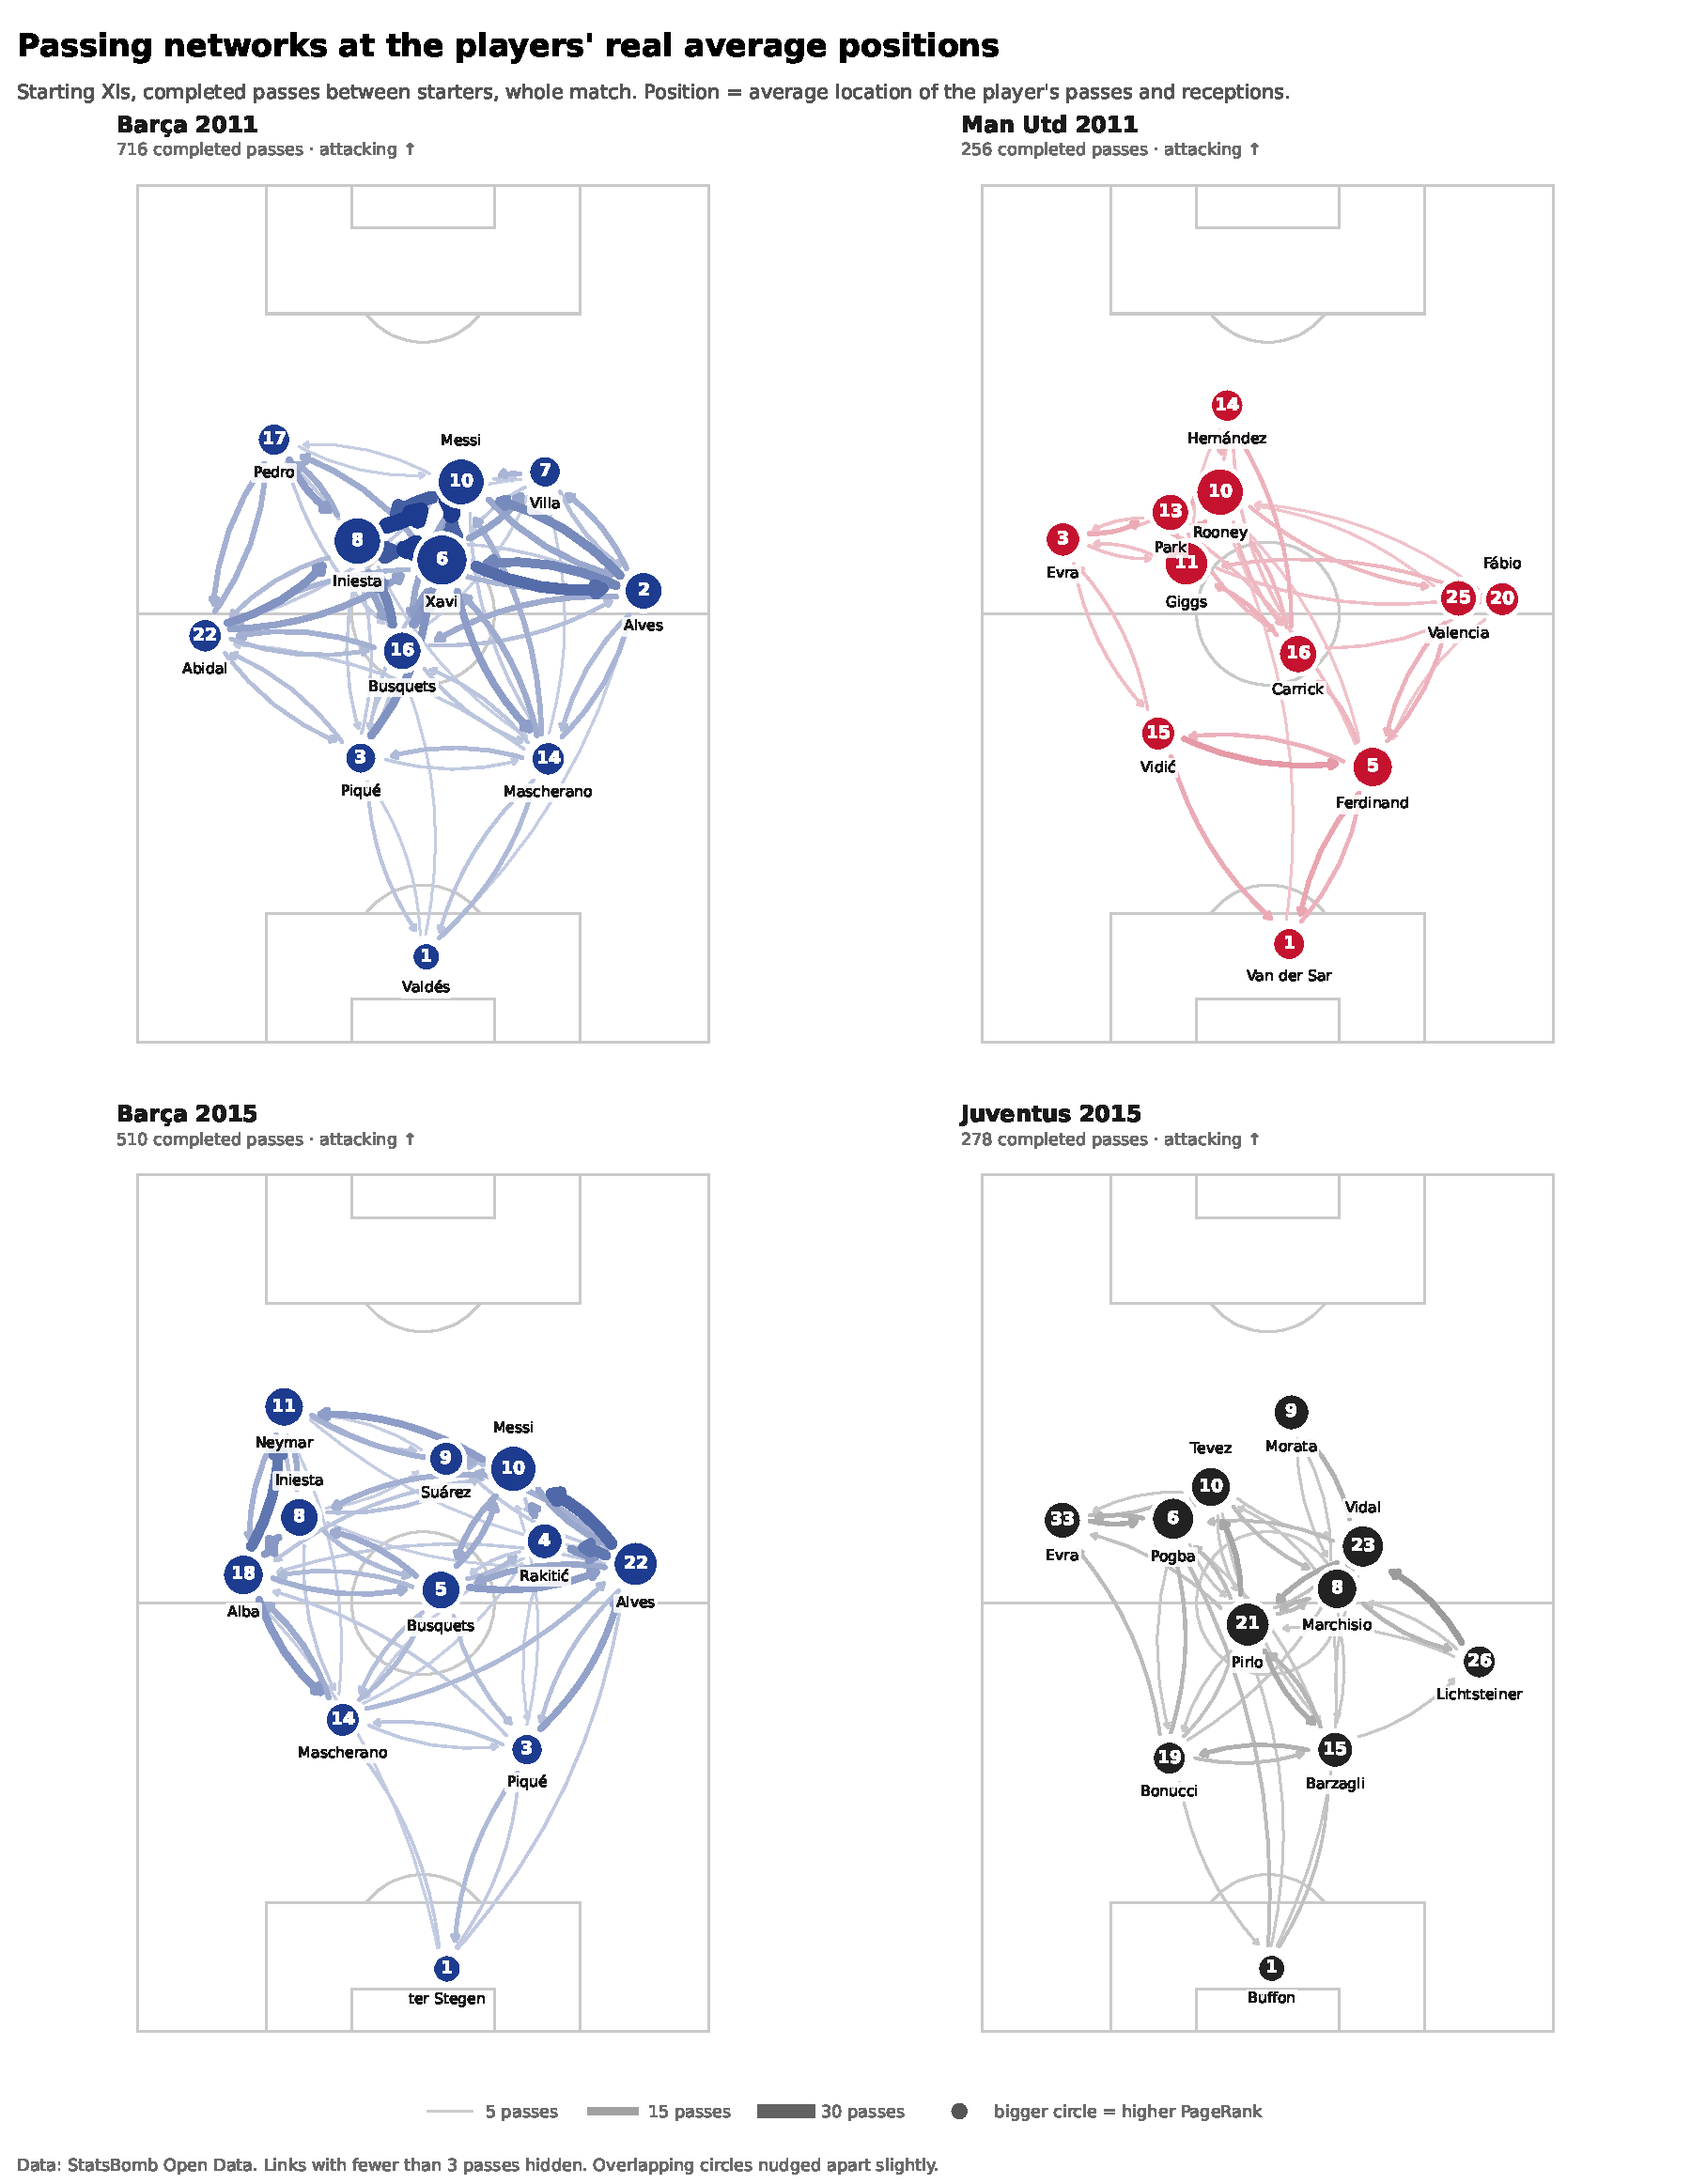
\includegraphics[width=0.93\textwidth]{sb_networks.pdf}
\caption{Passing networks at the players' real average positions (StatsBomb Open Data), attacking upwards. Circle size shows PageRank; links with fewer than three passes are hidden. Data: StatsBomb.}
\label{fig:sbnetworks}
\end{figure}

\paragraph{First half against second half.} Splitting each match at half-time (Table~\ref{tab:halves}, Figure~\ref{fig:halves}) shows how the games changed. In 2015, Barcelona completed 336 passes between starters in the first half but only 174 in the second. Meanwhile the share of Juventus's passes in the final third rose from 14\% to 25\%, as Juventus pushed for, and found, an equaliser. In 2011, Barcelona's dependence on Xavi fell in the second half (centralisation 0.56 to 0.35) as Messi became more involved. Messi scored the decisive second goal nine minutes after half-time.

\begin{table}[t]
\centering\small
\caption{First half against second half (StatsBomb). Final-third share = proportion of a team's completed passes that started in the attacking third.}
\label{tab:halves}
\begin{tabular}{lrrrlr}
\toprule
Team & Half & Passes & Final third & Top PageRank & Betweenness centralisation \\
\midrule
Barça 2011 & 1 & 387 & 24\% & Xavi, Iniesta & 0.559 \\
 & 2 & 329 & 25\% & Xavi, Messi & 0.349 \\
Man Utd 2011 & 1 & 139 & 29\% & Giggs, Rooney & 0.199 \\
 & 2 & 117 & 17\% & Rooney, Ferdinand & 0.266 \\
Barça 2015 & 1 & 336 & 24\% & Alves, Messi & 0.273 \\
 & 2 & 174 & 28\% & Messi, Alves & 0.284 \\
Juventus 2015 & 1 & 138 & 14\% & Pirlo, Vidal & 0.298 \\
 & 2 & 140 & 25\% & Tevez, Pogba & 0.102 \\
\bottomrule
\end{tabular}
\end{table}


\begin{figure}[t]
\centering
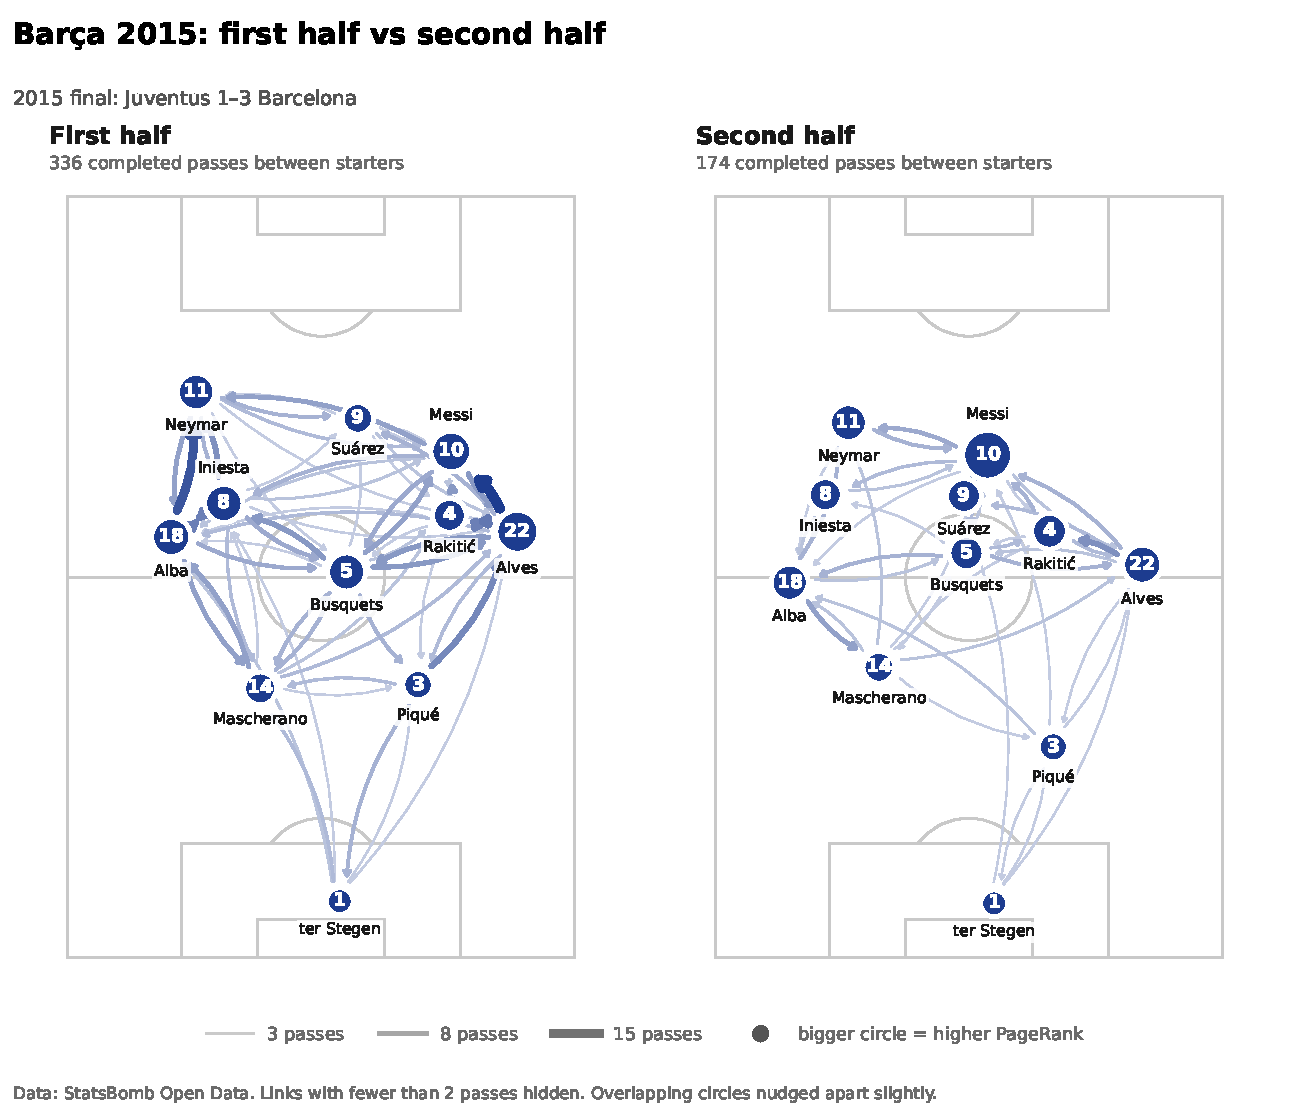
\includegraphics[width=0.8\textwidth]{sb_halves_barca2015.pdf}
\caption{Barcelona 2015 by half (StatsBomb). The second-half network is much thinner as Juventus took more of the ball. Data: StatsBomb.}
\label{fig:halves}
\end{figure}

%=====================================================================
\section{Probability: the Poisson model}\label{sec:poisson}
%=====================================================================

\subsection{From Bernoulli to Poisson}

Divide a 90-minute match into $n$ short intervals. Suppose that in each interval a team scores with a small probability $p$, independently of the other intervals, and cannot score twice in the same interval. Each interval is then a \textbf{Bernoulli trial}, with $P(1) = p$ and $P(0) = 1-p$, or $f(k;p) = p^k(1-p)^{1-k}$ for $k\in\{0,1\}$. The number of goals $X$ is a sum of $n$ independent Bernoulli trials, so it follows the \textbf{binomial distribution}
\[
P(X = k) = \binom{n}{k} p^k (1-p)^{n-k}.
\]
For example, with $n = 6$ periods of 15 minutes, scoring in exactly periods 3 and 6 has probability $p^2(1-p)^4$. There are $\binom{6}{2} = 15$ such arrangements, so $P(X=2) = 15\,p^2(1-p)^4$.

The restriction of one goal per interval disappears as the intervals shrink. Let $n\to\infty$ while keeping the expected number of goals $\lambda = np$ fixed. Then
\[
P(X=k) = \frac{n(n-1)\cdots(n-k+1)}{n^k}\cdot\frac{\lambda^k}{k!}\cdot\Big(1-\frac{\lambda}{n}\Big)^{n}\cdot\Big(1-\frac{\lambda}{n}\Big)^{-k}
\;\longrightarrow\; 1\cdot\frac{\lambda^k}{k!}\cdot e^{-\lambda}\cdot 1 ,
\]
since each factor $\frac{n-j}{n}\to 1$, $\big(1-\frac{\lambda}{n}\big)^n \to e^{-\lambda}$ and $\big(1-\frac{\lambda}{n}\big)^{-k}\to 1$. This is the \textbf{Poisson distribution},
\[
P(X = k) = \frac{\lambda^k e^{-\lambda}}{k!}, \qquad k = 0, 1, 2, \ldots,
\]
whose mean (and variance) is $\lambda$.

\subsection{Attack and defence}

Following Maher \cite{maher} and Spiegelhalter and Ng \cite{spiegelhalter}, the expected number of goals team $i$ scores against team $j$ is
\[
\lambda_{ij} = \bar g \cdot \alpha_i \cdot \delta_j, \qquad
\alpha_i = \frac{\text{goals scored per game by } i}{\bar g}, \qquad
\delta_j = \frac{\text{goals conceded per game by } j}{\bar g},
\]
where $\bar g$ is the average number of goals a team scores per game in the competition. $\alpha_i$ is team $i$'s \emph{attack strength}: $\alpha_i = 1.4$ means 40\% more goals than average. $\delta_j$ is team $j$'s \emph{defensive weakness}. Substituting shows that $\lambda_{ij}$ is simply (goals per game scored by $i$) $\times$ (goals per game conceded by $j$) $\div\ \bar g$. If the two teams' goals are independent Poisson variables with means $\lambda_B$ and $\lambda_O$, then
\[
P(\text{score } a\text{--}b) = \frac{\lambda_B^a e^{-\lambda_B}}{a!}\cdot\frac{\lambda_O^b e^{-\lambda_O}}{b!}, \qquad
P(\text{win}) = \sum_{a > b} P(a\text{--}b).
\]

\subsection{Two corrections}\label{sec:corrections}

\paragraph{One league average.} The 2018 essay used $\bar g = 1.31$ for goals scored and 1.59 for goals conceded (2010/11), and 1.33 and 1.58 (2014/15). This cannot be right. Every goal is scored by exactly one team and conceded by exactly one team, so over a whole competition
\[
\sum_{\text{teams}} \text{goals scored} = \sum_{\text{teams}} \text{goals conceded},
\]
and the two averages must be equal. From the group stage onwards both seasons had 125 matches, with 355 goals in 2010/11 and 361 in 2014/15. That gives $\bar g = 355/250 = 1.42$ and $361/250 = 1.44$ (version~A in Table~\ref{tab:poisson-finals}).

\paragraph{Do not use the result to predict itself.} The 2018 per-game figures are exact fractions of 13 games. For example, Barcelona's 2.31 goals per game in 2010/11 is $30/13$. So they include the final being predicted. Removing the final (3--1 in both years) leaves 12 games per finalist (version~B). In 2010/11 United had conceded only 4 goals in 12 games before the final, giving a defensive weakness of $\delta = 0.24$. Barcelona's expected goals then fall to 0.53, and the model makes United slight favourites (35\% against 24\%). In 2015, Barcelona remain favourites (38\% against 28\%). The 2018 model's apparent good sense came partly from already knowing the score.

\begin{table}[t]
\centering\small
\caption{The Poisson model for the two finals. $\lambda_B$ is Barcelona's expected goals and $\lambda_O$ the opponent's; win, draw and loss are from Barcelona's point of view, assuming independent Poisson scores.}
\label{tab:poisson-finals}
\begin{tabular}{llrrrrrrr}
\toprule
Final & Version & $\bar g$ & $\lambda_B$ & $\lambda_O$ & Win & Draw & Loss & $P(3\text{--}1)$ \\
\midrule
2011 & 2018 essay & 1.310 & 0.784 & 0.631 & 35.6\% & 37.9\% & 26.5\% & 1.23\% \\
2011 & A: one league average & 1.420 & 0.875 & 0.713 & 37.0\% & 35.3\% & 27.7\% & 1.63\% \\
2011 & B: A, final excluded & 1.415 & 0.530 & 0.707 & 24.0\% & 41.0\% & 35.1\% & 0.51\% \\
\addlinespace
2015 & 2018 essay & 1.330 & 1.160 & 0.704 & 46.7\% & 31.0\% & 22.3\% & 2.84\% \\
2015 & A: one league average & 1.444 & 1.270 & 0.766 & 48.3\% & 29.2\% & 22.5\% & 3.42\% \\
2015 & B: A, final excluded & 1.440 & 0.946 & 0.772 & 38.0\% & 33.6\% & 28.3\% & 1.95\% \\
\bottomrule
\end{tabular}
\end{table}


The probability of the exact score 3--1 is small in every version: between 0.5\% and 3.4\%. That is not evidence against the model on its own. Even the most likely score (0--0 in version B, both years) has a probability of only 18--29\%. A model has to be judged on many matches, which the next section does.

%=====================================================================
\section{Testing the model}\label{sec:test}
%=====================================================================

\subsection{Method}

Two finals cannot tell us whether the model works. I therefore predicted all \nKO{} knockout matches in \nSeasons{} Champions League seasons (2011/12--2023/24). Each prediction used only the results of that season played before the match: the group stage plus any earlier knockout games. The outcome is the result after 90 minutes: \nHome{} home wins, \nDraw{} draws and \nAway{} away wins. Finals, and the single-venue ties of 2019/20, are treated as neutral. Five forecasts are compared:
\begin{enumerate}
\item \textbf{Guess}: $1/3$ each for home win, draw and away win.
\item \textbf{Base rates}: the proportions of home wins, draws and away wins so far that season.
\item \textbf{The essay's model}, with the corrections of Section~\ref{sec:corrections}.
\item \textbf{The essay's model with home advantage}: $\bar g$ replaced by the average goals of home teams (for the home side) and of away teams (for the away side).
\item \textbf{A fitted Dixon--Coles model} \cite{dixoncoles}: $\log\lambda_{\text{home}} = \mu + h + a_i - d_j$ and $\log\lambda_{\text{away}} = \mu + a_j - d_i$, with attack $a$, defence $d$ and home advantage $h$ estimated by maximum likelihood. Because each team has only 6--12 earlier matches, the estimates are shrunk towards average by a normal prior with standard deviation 0.3. A correction factor $\tau$ adjusts the probabilities of 0--0, 1--0, 0--1 and 1--1, which plain Poisson models are known to get wrong:
\[
\tau(0,0) = 1-\lambda\mu\rho,\quad \tau(0,1) = 1+\lambda\rho,\quad \tau(1,0) = 1+\mu\rho,\quad \tau(1,1) = 1-\rho .
\]
\end{enumerate}

Forecasts are scored with the \textbf{ranked probability score} \cite{epstein, constantinou}, the standard measure for football, together with log loss and the Brier score. For forecast probabilities $(p_1,p_2,p_3)$ of home win, draw and away win, and the outcome $(o_1,o_2,o_3)$, one of which is 1,
\[
\text{RPS} = \frac{1}{2}\sum_{k=1}^{2}\Big(\sum_{j\le k}(p_j - o_j)\Big)^2 .
\]
It is lower for better forecasts, and it rewards a forecast that is ``close'': predicting a draw when the home team wins is less wrong than predicting an away win.

\subsection{Results}

\begin{table}[t]
\centering\small
\caption{Forecasting 371 Champions League knockout matches (2011/12--2023/24), each from the same season's earlier results. Lower is better for RPS, log loss and Brier score.}
\label{tab:modelcheck}
\begin{tabular}{lrrrr}
\toprule
Model & RPS & Log loss & Brier & Favourite won \\
\midrule
Guess 1/3 each & 0.2454 & 1.099 & 0.667 & -- \\
Home/draw/away rates so far & 0.2329 & 1.041 & 0.627 & 48.0\% \\
Essay's model (corrected averages) & 0.2467 & 1.106 & 0.659 & 46.6\% \\
Essay's model + home advantage & 0.2350 & 1.071 & 0.634 & 48.8\% \\
Fitted Dixon--Coles model & 0.2211 & 1.015 & 0.606 & 53.4\% \\
\bottomrule
\end{tabular}

\vspace{8pt}
\begin{tabular}{lrr}
\toprule
Difference in mean RPS & Estimate & 95\% bootstrap interval \\
\midrule
Essay's model $-$ base rates & $+0.0138$ & $[-0.0062,\ +0.0350]$ \\
Essay's model + home $-$ base rates & $+0.0022$ & $[-0.0158,\ +0.0213]$ \\
Dixon--Coles $-$ base rates & $-0.0118$ & $[-0.0208,\ -0.0017]$ \\
Adding home advantage & $-0.0116$ & $[-0.0180,\ -0.0053]$ \\
Dixon--Coles $-$ essay's model + home & $-0.0139$ & $[-0.0243,\ -0.0038]$ \\
\bottomrule
\end{tabular}
\end{table}


Table~\ref{tab:modelcheck} gives the results, with 95\% bootstrap intervals for the differences.
\begin{itemize}
\item \textbf{The essay's model is no better than the base rates.} Its mean RPS is slightly \emph{worse}, although the interval includes zero. Knowing only how often home teams usually win beats it.
\item \textbf{Home advantage is the biggest missing ingredient.} Adding it improves the essay's model clearly (the interval excludes zero).
\item \textbf{A fitted model does better still.} Dixon--Coles beats the base rates and the essay's model with home advantage, with both intervals excluding zero. The favourite won 53\% of the time under Dixon--Coles, against 47\% for the essay's model.
\end{itemize}

Figure~\ref{fig:calibration} shows why the essay's model struggles. It is \textbf{overconfident}. When it gave the home team about a 10\% chance, home teams actually won a third of the time. When it predicted a draw at over 40\%, fewer than one in ten of those matches were draws. Estimating team strengths from goals alone, from so few games, produces extreme values of $\alpha$ and $\delta$, just as United's $\delta = 0.24$ did in 2011. On average all three Poisson models predict more draws (\drawEssay{} for the essay's model, \drawDC{} for Dixon--Coles) than the \drawActual{} observed. That fits the idea that teams in two-legged knockout ties play for a result over the two legs, not for a draw in one match.

\begin{figure}[t]
\centering
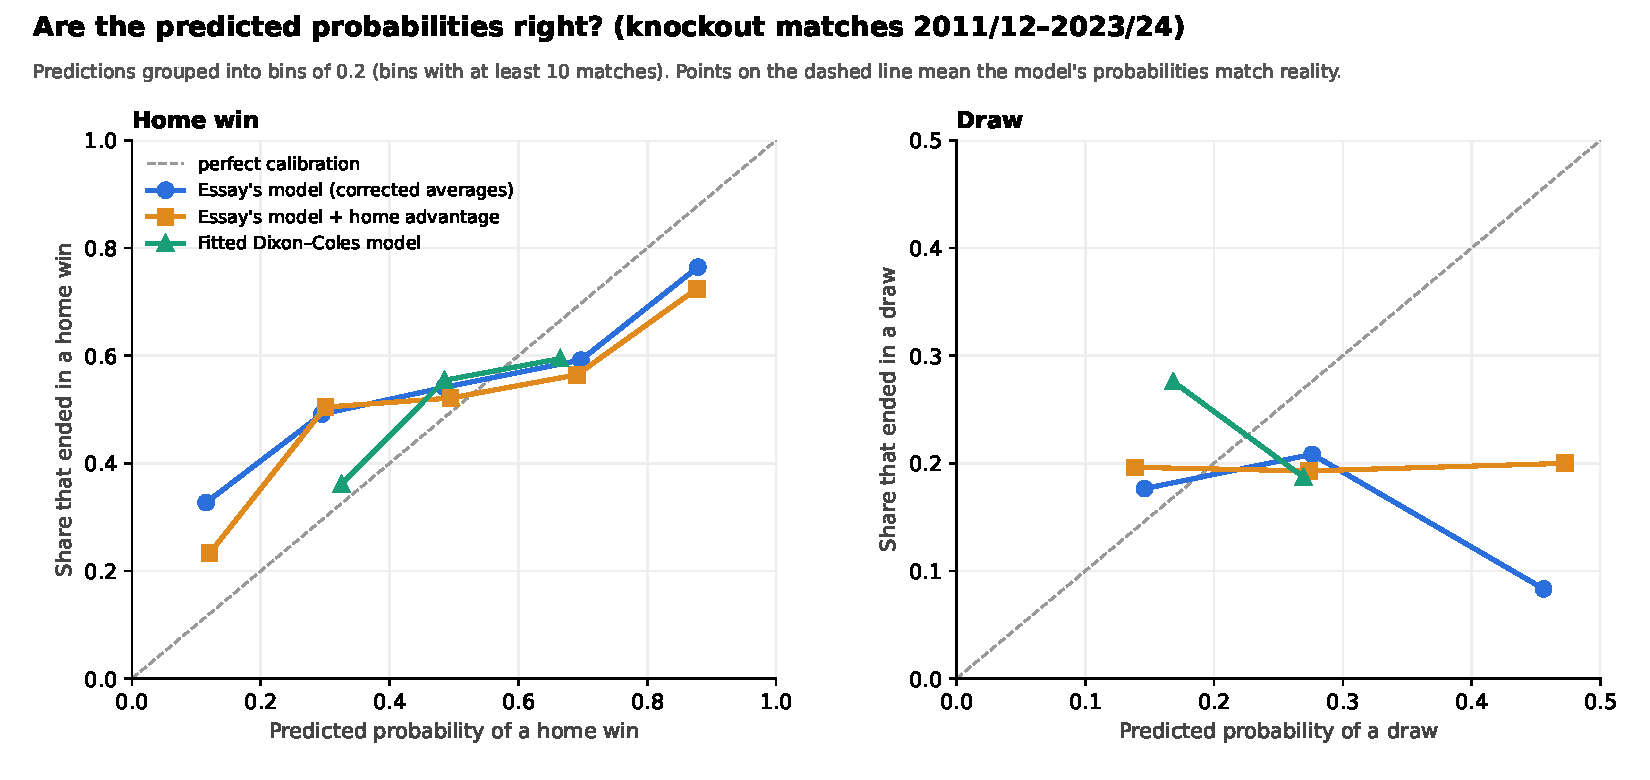
\includegraphics[width=\textwidth]{calibration.pdf}
\caption{Calibration: predicted probability against how often the event happened, for home wins (left) and draws (right). A well-calibrated model lies on the dashed line.}
\label{fig:calibration}
\end{figure}

%=====================================================================
\section{Expected goals: how good were the chances?}\label{sec:xg}
%=====================================================================

Goals are rare and noisy; chances are not. StatsBomb gives every shot an \textbf{expected-goals} value (xG): the probability that a shot from that position and situation is scored, estimated from many thousands of past shots. Adding a team's xG measures the quality of the chances it created, whatever the score.

To turn chances into result probabilities, I treat each attacking possession as a Bernoulli trial. Shots in the same possession, such as a shot and its rebound, are not independent. So a possession with shots of xG $q_1,\ldots,q_m$ scores with probability $1-\prod_{k}(1-q_k)$. A team's goals are then a sum of independent Bernoulli trials with different probabilities, and I simulate that sum 100{,}000 times. This asks: \emph{given the chances each team actually created, how often would this match end in each result?}

\begin{table}[t]
\centering\footnotesize\setlength{\tabcolsep}{4pt}
\caption{Shots and expected goals (Barcelona first). The simulated probabilities replay every chance 100{,}000 times; the last column is the pre-match Poisson forecast (final excluded, Table~\ref{tab:poisson-finals}).}
\label{tab:xg}
\begin{tabular}{lrrrrrrrr}
\toprule
Final & Shots & xG & Goals & Barça win & Draw & Opp.\ win & $P$(3--1) & Pre-match Barça win \\
\midrule
2011 & 22--4 & 1.93--0.30 & 3--1 & 80\% & 16\% & 4\% & 4.8\% & 24\% \\
2015 & 17--15 & 2.27--1.38 & 3--1 & 59\% & 23\% & 18\% & 10.8\% & 38\% \\
\bottomrule
\end{tabular}
\end{table}


\begin{figure}[t]
\centering
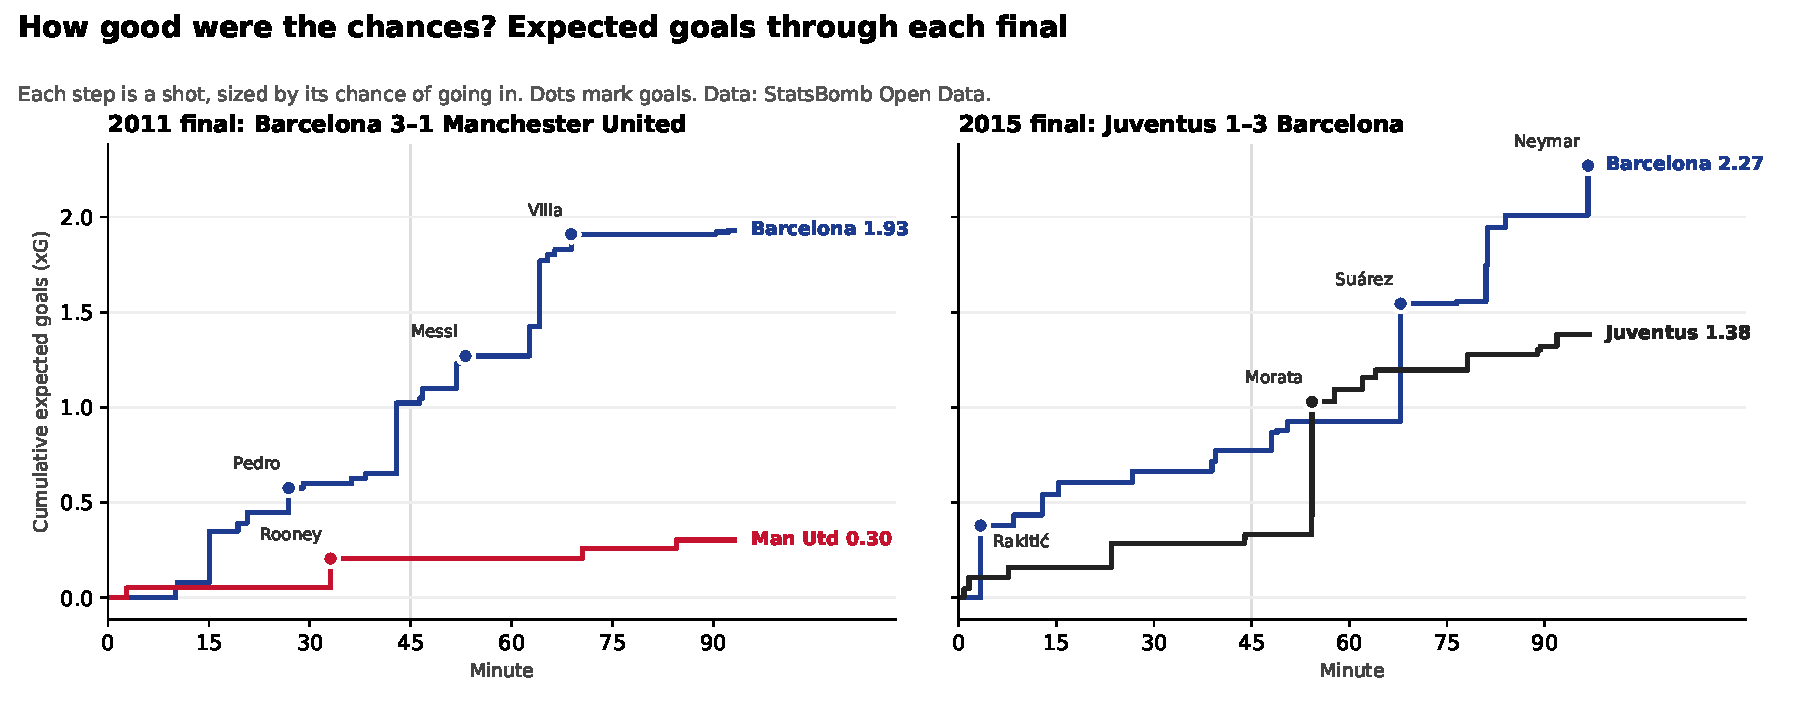
\includegraphics[width=\textwidth]{sb_xg_timeline.pdf}
\caption{Cumulative expected goals through each final (StatsBomb). Each step is a shot; dots mark goals. Data: StatsBomb.}
\label{fig:xg}
\end{figure}

The two finals look very different (Table~\ref{tab:xg}, Figure~\ref{fig:xg}). In 2011, Barcelona out-shot United 22 to 4 and created 1.93 xG to 0.30. United's goal came from one of only four shots. Given those chances Barcelona win 80\% of the time. Their dominance of the ball, which the networks show, turned directly into chances. The pre-match Poisson model, working only from goals in earlier games, gave Barcelona 24\%.

The 2015 final was closer: 2.27 xG to 1.38, and a 59\% chance of a Barcelona win. Rakiti\'c scored in the fourth minute. Morata's equaliser came from a 0.60 xG chance early in the second half, during the spell when Juventus took over the ball (Table~\ref{tab:halves}). Su\'arez restored the lead after 68 minutes, and Neymar scored in stoppage time. Here the Poisson and xG views agree more closely (38\% and 59\%), but only xG sees how the match unfolded.

%=====================================================================
\section{Linking the network to the chances}\label{sec:link}
%=====================================================================

The 2018 essay argued that the network analysis could explain the probability model's results, but it never connected the two. Event data make that connection possible. For each player I compute:
\begin{itemize}
\item \textbf{xGChain}: the total xG of every shot-ending possession the player was involved in;
\item \textbf{xGBuildup}: the same, but leaving out possessions in which the player took the shot or played the final pass. This measures contribution to the \emph{build-up}.
\end{itemize}
If the passing network captures something real, the most central passers should also be the main builders of chances. Table~\ref{tab:chain} compares each player's PageRank rank with their xGBuildup rank.

\begin{table}[t]
\centering\small
\caption{Who was involved in the chances? xGChain and xGBuildup for the top three players in each team, and the Spearman rank correlation between PageRank (StatsBomb network) and xGBuildup across the eleven starters.}
\label{tab:chain}
\begin{tabularx}{\textwidth}{lXXrr}
\toprule
Team & Highest xGChain & Highest xGBuildup & $\rho$ & $p$ \\
\midrule
Barça 2011 & Messi 1.80, Busquets 1.65, Xavi 1.55 & Busquets 1.57, Abidal 1.06, Xavi 1.04 & $0.31$ & 0.36 \\
Man Utd 2011 & Rooney 0.30, Giggs 0.26, Carrick 0.26 & Carrick 0.21, Giggs 0.20, Fábio 0.15 & $0.35$ & 0.29 \\
Barça 2015 & Messi 2.02, Alves 1.66, Rakitić 1.59 & Alves 1.43, Messi 1.33, Mascherano 1.08 & $0.65$ & 0.03 \\
Juventus 2015 & Marchisio 0.95, Morata 0.94, Tevez 0.87 & Marchisio 0.75, Lichtsteiner 0.20, Vidal 0.18 & $0.06$ & 0.85 \\
\bottomrule
\end{tabularx}
\end{table}


For Barcelona in 2015 the link is clear ($\rho = 0.65$, $p = 0.03$). Alves and Messi, the two most central players in the network, were also the two leading builders of chances. The right-sided play found in the network turned into chances. For Barcelona in 2011 the correlation is weaker (0.31). Busquets and Abidal contributed more to the build-up of chances than their network positions suggest, while Xavi, the network's hub, is third. For Juventus there is no relationship. Almost all of their build-up passed through Marchisio, who was not their most central passer. With eleven players per team, these correlations are only suggestive, but they are the first direct test of the claim that a team's passing structure explains its attacking output.

%=====================================================================
\section{Limitations}\label{sec:limitations}
%=====================================================================

\begin{itemize}
\item \textbf{Two matches.} The network results describe two finals and four team performances. They illustrate what the methods can show; they do not establish general laws about Barcelona or about football.
\item \textbf{Whole-match networks.} Aggregating over 90 minutes hides changes of tactics and game state. The half-by-half split is a first step; a finer split, for example into ten-minute windows or before and after each goal, would need more careful handling of small numbers.
\item \textbf{Completed passes only.} Failed passes, carries and dribbles are not in the networks. Nor is the opponent: a pass under pressure counts the same as an easy one.
\item \textbf{Starters only.} Substitutes are excluded, as in 2018. In these finals no substitution was made before the 69th minute, so the effect is small.
\item \textbf{The random-network baseline ignores the pitch.} A goalkeeper is as likely to pass to a striker as to a centre-back. Any real team will look unusually structured against it. A stricter baseline would keep players' positions.
\item \textbf{Small samples for the probability model.} Team strengths come from 6--12 earlier games. This is why the essay's model is overconfident, and it limits any model based on goals. Shots or xG from earlier games would give more stable strengths, but they are not in the openfootball data.
\item \textbf{xG is itself a model.} StatsBomb's xG values are estimates, and the simulation assumes that different possessions are independent.
\end{itemize}

%=====================================================================
\section{Conclusion}\label{sec:conclusion}
%=====================================================================

\emph{How can the knowledge of probability and network theory help quantitatively and qualitatively analyse a football team?} Eight years later, my answer has three parts.

\textbf{Network theory describes \emph{how} a team plays, but only if the mathematics matches the football.} Once more passes mean a shorter distance, the measures agree with what the pictures show. They also quantify things the eye can only guess at. Barcelona in 2011 were not a team without a centre. They were built around Xavi, whose removal would cost 14\% of their passing efficiency, far more than any other player on either side. In 2015 they had become a two-sided team, with Alves and Messi at its hub. Random-network comparisons and resampling show which patterns are real (the passing units, the concentration of passes on particular links, Xavi's role) and which are fragile (the order of Rooney and Ferdinand, or of Alves and Messi).

\textbf{A Poisson model of goals is a useful starting point, but on its own it is a weak forecaster.} Correctly applied and tested on \nKO{} matches, the model from the original essay does no better than the season's home, draw and away rates. Adding home advantage and fitting the model properly both help, but goals are too rare for a handful of earlier matches to reveal a team's true strength.

\textbf{The two approaches are strongest together, joined by better data.} Expected goals measure the quality of chances rather than the number of goals. They show that Barcelona's control of the ball in 2011 turned into a dominant set of chances, and that the 2015 final was closer than 3--1 suggests. Linking players' network positions to the chances they helped create gives the first direct test of the 2018 essay's claim that the network explains the goals. For Barcelona in 2015, it did.

The 2018 essay ended by saying that ``more work needs to be done in this field for it to ultimately be proved successful''. This edition does some of that work. Its main lesson is the one I would give my eighteen-year-old self: understand what a formula or a software function assumes before trusting its output, and test a model on more than the examples it was built from.

%=====================================================================
\section*{Reproducibility}\label{sec:reproducibility}
\addcontentsline{toc}{section}{Reproducibility}
%=====================================================================
All code is in the \texttt{recalc/} folder of the repository that accompanies this paper, and the tables are generated by \texttt{paper/make\_tables.py}. \texttt{recalculate.py} reproduces the 2018 values and computes the corrected measures. \texttt{network\_extra.py} contains the team measures, red-card test, passing units, random networks and bootstrap. \texttt{model\_check.py} runs the forecasting test. \texttt{statsbomb\_analysis.py} contains the event-data analysis; its data are downloaded by \texttt{fetch\_statsbomb.py}. Random seeds are fixed, so rerunning the scripts reproduces every number.

\paragraph{Data acknowledgements.} Passing tables: Opta, as used in the 2018 essay. Event data: StatsBomb Open Data \cite{statsbomb}. StatsBomb asks that any published work using its data credits StatsBomb as the source and displays its logo. Match results: openfootball (public domain) \cite{openfootball}.

%=====================================================================
\begin{thebibliography}{99}\small
\bibitem{louvain} V.~D. Blondel, J.-L. Guillaume, R.~Lambiotte and E.~Lefebvre, Fast unfolding of communities in large networks, \emph{Journal of Statistical Mechanics} (2008) P10008.
\bibitem{brandes} U.~Brandes, A faster algorithm for betweenness centrality, \emph{Journal of Mathematical Sociology} 25 (2001) 163--177.
\bibitem{brin} S.~Brin and L.~Page, The anatomy of a large-scale hypertextual web search engine, \emph{Computer Networks and ISDN Systems} 30 (1998) 107--117.
\bibitem{constantinou} A.~C. Constantinou and N.~E. Fenton, Solving the problem of inadequate scoring rules for assessing probabilistic football forecast models, \emph{Journal of Quantitative Analysis in Sports} 8 (2012).
\bibitem{dixoncoles} M.~J. Dixon and S.~G. Coles, Modelling association football scores and inefficiencies in the football betting market, \emph{Journal of the Royal Statistical Society C} 46 (1997) 265--280.
\bibitem{epstein} E.~S. Epstein, A scoring system for probability forecasts of ranked categories, \emph{Journal of Applied Meteorology} 8 (1969) 985--987.
\bibitem{fagiolo} G.~Fagiolo, Clustering in complex directed networks, \emph{Physical Review E} 76 (2007) 026107.
\bibitem{freeman} L.~C. Freeman, Centrality in social networks: conceptual clarification, \emph{Social Networks} 1 (1979) 215--239.
\bibitem{latora} V.~Latora and M.~Marchiori, Efficient behavior of small-world networks, \emph{Physical Review Letters} 87 (2001) 198701.
\bibitem{pena} J.~L\'opez Pe\~na and H.~Touchette, A network theory analysis of football strategies, in \emph{Sports Physics: Proceedings of the 2012 Euromech Physics of Sports Conference}, 2012. arXiv:1206.6904.
\bibitem{maher} M.~J. Maher, Modelling association football scores, \emph{Statistica Neerlandica} 36 (1982) 109--118.
\bibitem{newman} M.~E.~J. Newman, Modularity and community structure in networks, \emph{PNAS} 103 (2006) 8577--8582.
\bibitem{onnela} J.-P. Onnela, J.~Saram\"aki, J.~Kert\'esz and K.~Kaski, Intensity and coherence of motifs in weighted complex networks, \emph{Physical Review E} 71 (2005) 065103.
\bibitem{openfootball} openfootball, \emph{Champions League} results data, \url{https://github.com/openfootball/champions-league} (CC0).
\bibitem{spiegelhalter} D.~Spiegelhalter and Y.~L. Ng, Understanding uncertainty: football crazy, \emph{Plus Magazine}, 2009. \url{https://plus.maths.org/content/understanding-uncertainty-football-crazy}
\bibitem{statsbomb} StatsBomb, \emph{StatsBomb Open Data}, \url{https://github.com/statsbomb/open-data}.
\end{thebibliography}

\appendix
\section{Passing tables}\label{app:matrices}
The four passing tables used throughout, transcribed from the 2018 essay (Opta).

\begin{table}[p]
\centering\small\setlength{\tabcolsep}{3.5pt}
\caption{Completed passes between starters, Barça 2011 (Opta, as used in the 2018 essay). Row = passer, column = receiver.}
\label{tab:matrix-0}
\begin{tabular}{l*{11}{r}}
\toprule
From / to & \rotatebox{70}{Valdés} & \rotatebox{70}{Piqué} & \rotatebox{70}{Mascherano} & \rotatebox{70}{Alves} & \rotatebox{70}{Abidal} & \rotatebox{70}{Xavi} & \rotatebox{70}{Busquets} & \rotatebox{70}{Iniesta} & \rotatebox{70}{Pedro} & \rotatebox{70}{Messi} & \rotatebox{70}{Villa} \\
\midrule
Valdés & 0 & 3 & 6 & 3 & 0 & 1 & 3 & 1 & 2 & 0 & 1 \\
Piqué & 4 & 0 & 5 & 1 & 6 & 16 & 6 & 4 & 2 & 1 & 1 \\
Mascherano & 5 & 7 & 0 & 8 & 4 & 11 & 6 & 1 & 0 & 9 & 2 \\
Alves & 1 & 1 & 7 & 0 & 0 & 17 & 9 & 4 & 0 & 17 & 8 \\
Abidal & 2 & 5 & 0 & 0 & 0 & 12 & 7 & 15 & 9 & 4 & 1 \\
Xavi & 2 & 5 & 15 & 22 & 8 & 0 & 12 & 33 & 11 & 23 & 11 \\
Busquets & 0 & 6 & 4 & 6 & 9 & 12 & 0 & 17 & 3 & 15 & 4 \\
Iniesta & 0 & 4 & 3 & 8 & 7 & 27 & 12 & 0 & 11 & 32 & 2 \\
Pedro & 0 & 0 & 1 & 0 & 9 & 2 & 2 & 15 & 0 & 3 & 0 \\
Messi & 0 & 2 & 3 & 11 & 1 & 32 & 10 & 25 & 3 & 0 & 3 \\
Villa & 0 & 0 & 1 & 6 & 0 & 4 & 2 & 2 & 1 & 7 & 0 \\
\bottomrule
\end{tabular}
\end{table}

\begin{table}[p]
\centering\small\setlength{\tabcolsep}{3.5pt}
\caption{Completed passes between starters, Man Utd 2011 (Opta, as used in the 2018 essay). Row = passer, column = receiver.}
\label{tab:matrix-1}
\begin{tabular}{l*{11}{r}}
\toprule
From / to & \rotatebox{70}{Van der Sar} & \rotatebox{70}{Evra} & \rotatebox{70}{Ferdinand} & \rotatebox{70}{Vidić} & \rotatebox{70}{Fábio} & \rotatebox{70}{Giggs} & \rotatebox{70}{Park} & \rotatebox{70}{Valencia} & \rotatebox{70}{Carrick} & \rotatebox{70}{Rooney} & \rotatebox{70}{Hernández} \\
\midrule
Van der Sar & 0 & 1 & 6 & 1 & 2 & 1 & 1 & 2 & 1 & 4 & 0 \\
Evra & 0 & 0 & 1 & 4 & 0 & 4 & 6 & 0 & 2 & 6 & 1 \\
Ferdinand & 7 & 2 & 0 & 6 & 0 & 1 & 5 & 6 & 5 & 3 & 0 \\
Vidić & 7 & 4 & 10 & 0 & 0 & 2 & 2 & 0 & 2 & 1 & 0 \\
Fábio & 0 & 0 & 3 & 0 & 0 & 5 & 0 & 4 & 0 & 3 & 0 \\
Giggs & 0 & 4 & 2 & 2 & 4 & 0 & 5 & 2 & 1 & 7 & 2 \\
Park & 0 & 4 & 0 & 2 & 1 & 3 & 0 & 1 & 5 & 6 & 1 \\
Valencia & 1 & 0 & 6 & 1 & 3 & 1 & 0 & 0 & 1 & 3 & 0 \\
Carrick & 2 & 1 & 1 & 1 & 4 & 6 & 1 & 1 & 0 & 5 & 6 \\
Rooney & 0 & 2 & 1 & 2 & 1 & 8 & 5 & 5 & 5 & 0 & 4 \\
Hernández & 0 & 0 & 0 & 0 & 0 & 3 & 1 & 1 & 3 & 4 & 0 \\
\bottomrule
\end{tabular}
\end{table}

\begin{table}[p]
\centering\small\setlength{\tabcolsep}{3.5pt}
\caption{Completed passes between starters, Barça 2015 (Opta, as used in the 2018 essay). Row = passer, column = receiver.}
\label{tab:matrix-2}
\begin{tabular}{l*{11}{r}}
\toprule
From / to & \rotatebox{70}{ter Stegen} & \rotatebox{70}{Piqué} & \rotatebox{70}{Mascherano} & \rotatebox{70}{Alba} & \rotatebox{70}{Alves} & \rotatebox{70}{Busquets} & \rotatebox{70}{Iniesta} & \rotatebox{70}{Rakitić} & \rotatebox{70}{Messi} & \rotatebox{70}{Neymar} & \rotatebox{70}{Suárez} \\
\midrule
ter Stegen & 0 & 5 & 3 & 5 & 3 & 0 & 2 & 0 & 1 & 0 & 2 \\
Piqué & 7 & 0 & 5 & 4 & 12 & 0 & 1 & 2 & 2 & 0 & 1 \\
Mascherano & 1 & 4 & 0 & 10 & 8 & 7 & 2 & 3 & 1 & 3 & 1 \\
Alba & 1 & 0 & 13 & 0 & 1 & 9 & 14 & 0 & 0 & 21 & 4 \\
Alves & 0 & 6 & 1 & 4 & 0 & 10 & 1 & 21 & 25 & 0 & 9 \\
Busquets & 2 & 6 & 6 & 6 & 16 & 0 & 9 & 7 & 9 & 0 & 2 \\
Iniesta & 0 & 1 & 4 & 14 & 3 & 7 & 0 & 2 & 7 & 10 & 2 \\
Rakitić & 0 & 3 & 3 & 2 & 14 & 7 & 2 & 0 & 12 & 1 & 1 \\
Messi & 0 & 2 & 0 & 5 & 10 & 10 & 9 & 7 & 0 & 12 & 6 \\
Neymar & 0 & 0 & 1 & 8 & 3 & 2 & 7 & 1 & 10 & 0 & 4 \\
Suárez & 0 & 1 & 0 & 0 & 4 & 1 & 2 & 3 & 7 & 4 & 0 \\
\bottomrule
\end{tabular}
\end{table}

\begin{table}[p]
\centering\small\setlength{\tabcolsep}{3.5pt}
\caption{Completed passes between starters, Juventus 2015 (Opta, as used in the 2018 essay). Row = passer, column = receiver.}
\label{tab:matrix-3}
\begin{tabular}{l*{11}{r}}
\toprule
From / to & \rotatebox{70}{Buffon} & \rotatebox{70}{Barzagli} & \rotatebox{70}{Bonucci} & \rotatebox{70}{Lichtsteiner} & \rotatebox{70}{Evra} & \rotatebox{70}{Pogba} & \rotatebox{70}{Marchisio} & \rotatebox{70}{Pirlo} & \rotatebox{70}{Vidal} & \rotatebox{70}{Tevez} & \rotatebox{70}{Morata} \\
\midrule
Buffon & 0 & 3 & 1 & 2 & 1 & 3 & 3 & 4 & 0 & 2 & 0 \\
Barzagli & 2 & 0 & 6 & 3 & 0 & 4 & 2 & 6 & 3 & 0 & 1 \\
Bonucci & 3 & 6 & 0 & 2 & 4 & 4 & 1 & 3 & 3 & 0 & 1 \\
Lichtsteiner & 1 & 1 & 0 & 0 & 0 & 1 & 2 & 3 & 12 & 2 & 1 \\
Evra & 0 & 0 & 1 & 0 & 0 & 8 & 1 & 2 & 3 & 5 & 0 \\
Pogba & 0 & 1 & 3 & 1 & 7 & 0 & 2 & 3 & 1 & 4 & 2 \\
Marchisio & 0 & 0 & 6 & 6 & 0 & 1 & 0 & 6 & 4 & 3 & 3 \\
Pirlo & 0 & 9 & 3 & 1 & 6 & 5 & 5 & 0 & 3 & 9 & 1 \\
Vidal & 0 & 5 & 0 & 2 & 2 & 4 & 3 & 8 & 0 & 0 & 7 \\
Tevez & 0 & 1 & 1 & 0 & 3 & 3 & 5 & 3 & 4 & 0 & 5 \\
Morata & 0 & 0 & 1 & 1 & 1 & 1 & 2 & 1 & 0 & 2 & 0 \\
\bottomrule
\end{tabular}
\end{table}


\end{document}
